% !Mode:: "TeX:UTF-8"
% !TEX program  = xelatex
\documentclass[withoutpreface,bwprint]{cumcmthesis} 
%'''
\usepackage{amsmath}   % Package for math files
\usepackage{txfonts}
\usepackage{graphicx}  % Place figures
\usepackage{caption}   % Place captions in tables and figures
\usepackage{subcaption}% 
\usepackage{placeins}  % \FloatBarrier so figures can't float beyond some point in text
\usepackage{fullpage}  % Uses more of the page
\usepackage{float}     % Able to make figures and tables float
%表格自动生成
\usepackage{subfloat}
\usepackage{subcaption} 
\usepackage{subfiles}  
\usepackage{hyperref} 
 % Ability to click on references like equations, figures, sections etc. \ref{eq:my_eq} clickable
\usepackage{placeins}  
% \FloatBarrier so figures can't float beyond some point in text
\usepackage[T1]{fontenc} 
%英文字体定义
\usepackage{setspace}
\usepackage{fontspec}

%''' 
%以上为宏包的引用


%'''
\renewcommand {\thetable} {\thechapter{}.\arabic{table}}
%表格根据章节自动命名
\renewcommand {\thefigure} {\thechapter{}.\arabic{figure}}
%图片根据章节自动命名
\numberwithin{figure}{section}
\numberwithin{table}{section}
\numberwithin{equation}{section}
%以上三个皆控制重命名
\newcommand{\figref}[1]{\figurename~\ref{#1}} 
%Nice reference to figures

\usepackage[framemethod=TikZ]{mdframed}
\usepackage{url}   % 网页链接
\usepackage{subcaption} % 子标题
\renewcommand{\contentsname}{Contents}
\renewcommand{\listfigurename}{List of Figures}
\renewcommand{\listtablename}{List of Tables}
\renewcommand{\indexname}{Index}
\renewcommand{\figurename}{Figure}
\renewcommand{\tablename}{Table}
\renewcommand{\refname}{References}
\usepackage{tocloft}
\usepackage{fancyhdr} 
%'''
%以上为renewcommand的使用
%页面格式编辑
\geometry{top=2.54cm, bottom=2.54cm, left=2.54cm, right=2.54cm, headheight=15pt}
%%以下部分编辑页眉与页脚
%\pagestyle{fancy}
%\fancyhf{} % 清除所有的页眉和页脚
%\setlength{\headheight}{15pt} % 增加页眉的高度
%\setlength{\headsep}{25pt}    % 增加页眉和正文之间的距离
%\fancyhead[R]{Student Name: Zhan Ruixin}
%\fancyhead[L]{Preliminary Report (ECM3175)} % 页眉左侧
%\fancyfoot[C]{\thepage} % 底部中央页码
%\renewcommand{\headrulewidth}{0pt} % 不显示页眉线
%\renewcommand{\footrulewidth}{0pt} % 不显示页脚线

%以下编辑为Final report设置

%% 章节标题定义
\usepackage{titlesec}
\titleformat{\section}
{\fontsize{16}{18.4}\selectfont\bfseries\fontspec{Arial}}{\thesection}{1em}{}
\titleformat{\subsection}
{\fontsize{14}{21}\selectfont\bfseries\itshape\fontspec{Cambria}}{\thesubsection}{1em}{}
\titleformat{\subsubsection}
{\fontsize{14}{21}\selectfont\bfseries\itshape\fontspec{Cambria}}{\thesubsection}{1em}{}
\titlespacing*{\section}
{0pt}{12pt plus 4pt minus 2pt}{6pt plus 2pt minus 2pt}
\titlespacing*{\subsection}
{0.63cm}{6pt plus 4pt minus 2pt}{6pt plus 2pt minus 2pt}
\titlespacing*{\subsubsection}
{0.63cm}{6pt plus 4pt minus 2pt}{6pt plus 2pt minus 2pt}

%%目录
% 标题格式
\renewcommand{\cfttoctitlefont}{\bfseries\fontsize{16}{19}\selectfont\Arial}
\renewcommand{\cftaftertoctitle}{\vspace{12pt}\hspace*{\fill}}
% 目录项格式
\renewcommand{\cftsecfont}{\fontsize{11}{13}\selectfont}
\renewcommand{\cftsecpagefont}{\fontsize{11}{1}\selectfont}
\renewcommand{\cftsubsubsecfont}{\fontsize{11}{13}\selectfont}
\renewcommand{\cftsubsecindent}{0.39cm}
\renewcommand{\cftsubsubsecindent}{0.8cm} 
% 调整目录行距
% 调整目录行距和段前后距
\setlength{\cftbeforesecskip}{10pt}
\setlength{\cftbeforesubsecskip}{10pt}
\setlength{\cftbeforesubsubsecskip}{10pt}
\setlength{\cftbeforetoctitleskip}{0pt}
\setlength{\cftaftertoctitleskip}{10pt}
% 重命名
\renewcommand{\contentsname}{Table of Contents}

%%
% 设置“References”标题的格式

% 设置参考文献标题 "References"
%\titleformat{\section}
%{\normalfont\bfseries\fontsize{18}{22}\selectfont\fontfamily{phv}\selectfont}
%{\thesection}{1em}{}
%\titlespacing*{\section}{0pt}{12pt}{12pt}
%
%% 设置参考文献列表的样式
%\renewcommand{\cftsecfont}{\bfseries\fontsize{18}{22}\selectfont\fontfamily{phv}\selectfont}
%\renewcommand{\cftsecpagefont}{\bfseries\fontsize{18}{22}\selectfont\fontfamily{phv}\selectfont}


%以上为格式规定与包的引用,勿动。以下为正文内容,从标题开始

%标题
\title{Title}

\renewcommand{\headrulewidth}{0pt} % 不显示页眉线
\renewcommand{\footrulewidth}{0pt} % 不显示页脚线\left( 
\begin{document}
 \maketitle
%英文摘要
\renewcommand{\abstractname}{Abstract}
\renewcommand{\keywords}{\textbf{Keywords:}}
\begin{abstract}
\begin{spacing}{1.6}

%英文摘要内容
\end{spacing}
\large


%本实验包括两个部分,分别研究了理想气体在绝热过程和等温过程中的膨胀变化。在绝热过程中通过实验测量数据的计算热容比,结果为1.357,相比于理想情况(1.4)存在3.07%的误差。在等温过程中通过实验测量数据的计算体积比,结果为2.330,相比于理想情况(2.4615)存在9.28%的误差。两个实验结果都基本符合理论情况,仅存在较小的误差。由于两个结果都相较于理论情况偏小,因此这一误差可能由相似的原因导致。例如实际气体并非理想气体导致测量数据偏小,环境条件控制不精确等,并提供了一些解决方法。
\end{abstract}

%目录(前三行为目录格式调整)
%\cftsetindents{section}{0em}{2em}
%\cftsetindents{subsection}{2em}{3em}
%\cftsetindents{subsubsection}{4em}{4em}
\newpage
{
	\fontspec{Times New Roman}
	\tableofcontents
}
\newpage

%
%以下部分为正文内容
\pagenumbering{arabic}
\section{Introduction and background}
\label{sec:introduction}


\subsection{Introduction}

\subsubsection{Project Overview}

This project addresses the critical task of optimizing the cutting parameters of a biological tissue slicer, an essential instrument in biomedical research and clinical diagnostics. The aim is to enhance the precision and efficiency of tissue sample preparation by identifying the optimal slicing conditions. Through the collection of tissue samples under various cutting parameters and subsequent artificial image classification, this study employs deep learning techniques to analyze and predict the most effective slicing parameters. This endeavor not only promises to improve the quality of tissue samples for microscopic examination but also to streamline the workflow in laboratories, thereby contributing to the advancement of biological and medical sciences.
% 这个项目解决了生物组织切片仪的关键任务,这是生物医学研究和临床诊断中的一个重要仪器。其目标是通过确定最佳切片条件来提高组织样本制备的精确性和效率。通过收集在不同切割参数下的组织样本,并进行人工图像分类,本研究采用深度学习技术来分析和预测最有效的切片参数。这个努力不仅有望改善显微镜检查的组织样本质量,还有望简化实验室的工作流程,从而促进生物和医学科学的进步。
\subsubsection{Objectives}

\begin{enumerate}
    \item Collect a comprehensive dataset of tissue samples sliced under different parameters.
    \item Employ artificial image classification to categorize the quality and characteristics of these samples.
    \item Develop and train a deep learning model capable of assessing tissue sample quality.
    \item Use the model's insights to determine the optimal cutting parameters for the tissue slicer.
    \item Validate the model's predictions through empirical testing and refinement.
\end{enumerate}

% \item 收集在不同参数下切割的组织样本的全面数据集。
% \item 使用人工图像分类来对这些样本的质量和特征进行分类。
% \item 开发和训练一个能够评估组织样本质量的深度学习模型。
% \item 利用模型的见解来确定组织切片仪的最佳切割参数。
% \item 通过实证测试和改进来验证模型的预测结果。
% \end{enumerate}

\subsubsection{Structure of the Report}

This project is organized into the following chapters, each designed to systematically explore the research background, methodologies, experimental work, results presentation, discussions and conclusions, as well as considerations for project management, sustainability, and health and safety:

\textbf{Introduction and Background} - This chapter outlines the project's objectives, goals, and structural arrangement. It provides a brief introduction to the motivation and necessity for the research, along with the technical protocols and specifications adopted.

\textbf{Literature Review} - An in-depth discussion on the use of biological tissue slicers, image classification, and deep learning in the preparation of biological samples. This section positions the current study within the context of existing research.

\textbf{Methodology and Theory} - Detailed descriptions of the experimental methods, theoretical frameworks, and the specific plans for data collection and processing are presented here.

\textbf{Experimental Work/Analytical Investigation/Design} - Describes the detailed steps of experimental design, implementation, and analytical investigation. It elaborates on the strategies and methods adopted to achieve the project's objectives.

\textbf{Presentation of Experimental or Analytical Results/Descriptions of Final Constructed Product} - This chapter showcases the experimental data, analysis results, or the final design product, providing detailed accounts of the experimental or design outcomes.

\textbf{Discussion and Conclusions} - The results are analyzed, and their scientific significance and practical value are discussed. This chapter also offers the research conclusions and suggests potential directions for future studies.

\textbf{Project Management, Consideration of Sustainability and Health and Safety} - Discusses strategies for project management, sustainability issues, and health and safety measures to ensure the research work is conducted efficiently and safely.

\textbf{References} - Lists all the bibliographic materials cited, supporting the research and providing the basis for the study.
% 本项目分为以下几个章节,每个章节都旨在系统地探索研究背景、方法论、实验工作、结果展示、讨论和结论,以及项目管理、可持续性和健康安全方面的考虑:

% \textbf{引言和背景} - 本章概述了项目的目标、目标和结构安排。它简要介绍了研究的动机和必要性,以及采用的技术协议和规范。

% \textbf{文献综述} - 对生物组织切片、图像分类和深度学习在生物样本制备中的应用进行深入讨论。本节将当前研究定位于现有研究的背景下。

% \textbf{方法和理论} - 详细描述了实验方法、理论框架以及数据收集和处理的具体计划。

% \textbf{实验工作/分析调查/设计} - 描述了实验设计、实施和分析调查的详细步骤。详细阐述了实现项目目标所采用的策略和方法。

% \textbf{实验或分析结果展示/最终构建产品描述} - 本章展示了实验数据、分析结果或最终设计产品,详细描述了实验或设计结果。

% \textbf{讨论和结论} - 对结果进行分析,讨论其科学意义和实际价值。本章还提供研究结论,并提出未来研究的潜在方向。

% \textbf{项目管理、可持续性和健康安全考虑} - 讨论项目管理策略、可持续性问题和健康安全措施,以确保研究工作的高效和安全进行。

% \textbf{参考文献} - 列出所有引用的文献资料,支持研究并为研究提供基础。

\subsubsection{Assumptions and Technical Specifications}

The project is based on several key assumptions and technical protocols, which are:

\begin{enumerate}
    \item The consistency in tissue sample properties across different batches.
    \item The reliability and precision of the biological tissue slicer and imaging equipment.
    \item The adequacy of the deep learning model in interpreting complex biological image data.
\end{enumerate}
Technical specifications regarding the tissue slicer settings, image classification criteria, and deep learning architecture are detailed in \textbf{Methodology and Theory}.
% 该项目基于几个关键假设和技术协议,包括:

% \begin{enumerate}
%     \item 不同批次之间组织样本性质的一致性。
%     \item 生物组织切片仪和成像设备的可靠性和精确性。
%     \item 深度学习模型在解释复杂生物图像数据方面的充分性。
% \end{enumerate}
% 有关组织切片仪设置、图像分类标准和深度学习架构的技术规格详见方法和理论。

\subsection{Background}

\subsubsection{Importance of Tissue Sample Quality}

High-quality tissue samples are pivotal for accurate diagnosis and research. The quality of a tissue sample can significantly affect the results of histological analysis, making the optimization of slicing parameters a crucial endeavor.

\subsubsection{Advancements in Image Classification and Deep Learning}

Recent advancements in image classification and deep learning have opened new avenues for automating and enhancing the analysis of biological samples. By leveraging these technologies, it is possible to achieve greater accuracy and efficiency in identifying optimal tissue slicing parameters.

\subsubsection{Gap in Current Research}

While there have been significant strides in both biological sample preparation and computational analysis, a gap remains in integrating these approaches to optimize tissue slicing parameters. This project aims to bridge this gap by developing a predictive model that can guide the adjustment of slicing conditions for optimal outcomes.

% \subsection{背景}

% \subsubsection{组织样本质量的重要性}

% 高质量的组织样本对于准确的诊断和研究至关重要。组织样本的质量可以显著影响组织学分析的结果,因此优化切片参数是一项关键的工作。

% \subsubsection{图像分类和深度学习的进展}

% 图像分类和深度学习的最新进展为自动化和增强生物样本分析开辟了新的途径。通过利用这些技术,可以在识别最佳组织切片参数方面实现更高的准确性和效率。

% \subsubsection{当前研究中的差距}

% 尽管在生物样本制备和计算分析方面取得了重大进展,但在整合这些方法以优化组织切片参数方面仍存在差距。本项目旨在通过开发一个预测模型来填补这一差距,该模型可以指导调整切片条件以获得最佳结果。

\section{Literature review}

\subsection{Technical background to tissue slicing and image acquisition}

%组织切片和图像获取的技术背景   这里写切片机和显微镜的技术参数和采集手册及方法

\subsection{Image Classification for Tissue Analysis}

%用于组织分析的图像分类   这里写图像分类的技术背景和方法


\subsection{Deep Learning in Biomedical Applications}

%深度学习在生物医学应用中的应用   这里写深度学习的技术背景和方法

\subsection{Integration of Deep Learning for Optimizing Tissue Slicing Parameters}

%整合深度学习以优化组织切片参数   这里写深度学习在优化切片参数中的应用


\FloatBarrier % Now figures cannot float above section title




%theory
\section{Methodology and theory}
\label{sec:problem_description}

\subsection{计算机视觉-图像分割}

对于获取的图像数据,可以应用适当的图像预处理。在保持图像完整性和质量的前提下,可以实施某些处理以突出计算机识别的特征,并在一定程度上去除无关特征和噪声。这增强了后续深度学习模型的准确性。

图像分割是图像处理中的关键步骤,目的是将图像划分为几个有意义的区域以进行进一步的分析和处理。在关注生物组织产率的模型中,需要将生物切片分割为生物组织和石蜡区域,强调生物组织部分。

常见的图像分割算法包括边缘检测和阈值分割。

\subsubsection{边缘检测}
对于生物组织切片,质量的关键指标是切片边缘的清晰度。切片边缘的完整性和连续性可以反映样本是否存在质量问题。

有许多边缘检测的算法,如Sobel、Laplacian和Canny算子 \cite{3.1}。

\textbf{Sobel算子}是一种一阶差分算子,可以用来检测图像边缘 \cite{补充1}。假设有一个一维图像$f(x)$,其强度与像素坐标$x$的关系可以如图1所示。在\autoref{fig:original_function}中可以观察到,斜率在x=2.2附近最大,表明在这个点附近图像强度有突然的变化(存在边缘)。取其导数得到一阶导数$f'(x)$,如\autoref{fig:first_derivative}所示,其中导数的绝对值最大。Sobel算子利用这个特性来检测边缘。

\begin{figure}[htbp]
    \centering
    \begin{minipage}[b]{0.32\textwidth}
        \centering
        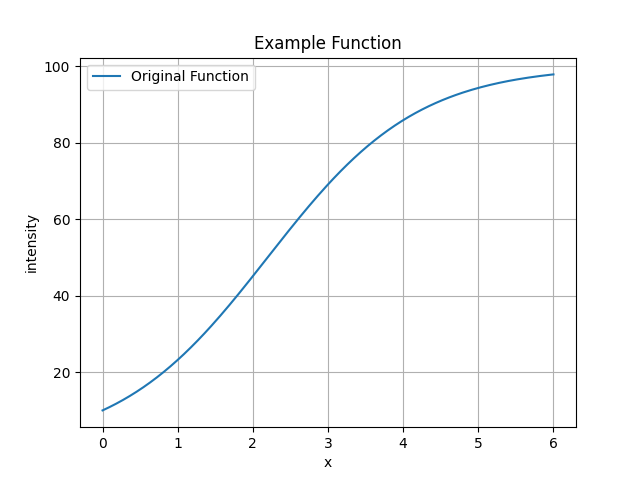
\includegraphics[width=\textwidth]{./fig/original_function.png}
        \caption{f(x)}
        \label{fig:original_function}
    \end{minipage}
    \begin{minipage}[b]{0.32\textwidth}
        \centering
        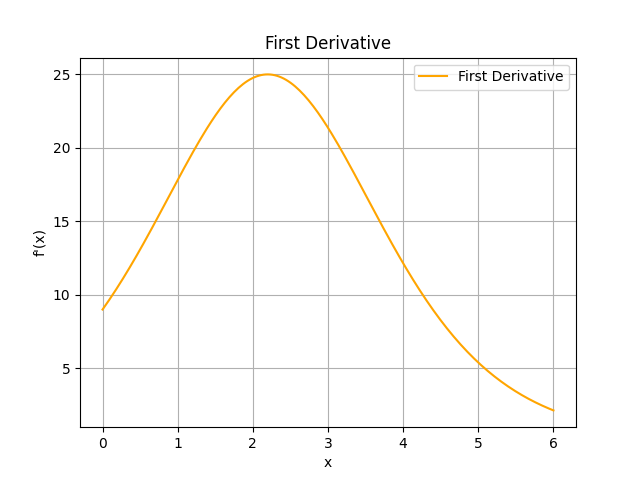
\includegraphics[width=\textwidth]{./fig/first_derivative.png}
        \caption{f'(x)}
        \label{fig:first_derivative}
    \end{minipage}
    \begin{minipage}[b]{0.32\textwidth}
        \centering
        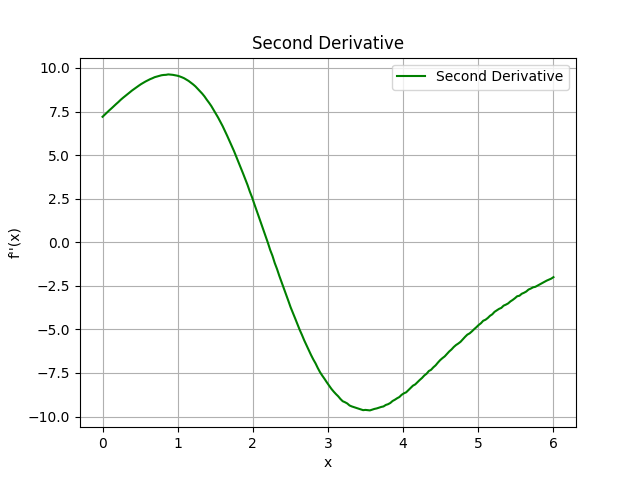
\includegraphics[width=\textwidth]{./fig/second_derivative.png}
        \caption{f''(x)}
        \label{fig:second_derivative}
    \end{minipage}
\end{figure}

\textbf{Laplacian算子}是一种二阶微分算子,其对图像的边缘检测效果较好。它是对sobel算子再进行一次求导得出。在2D图像中,Laplacian算子的定义如下:
\begin{equation}
    \nabla^2 f = \frac{\partial^2 f}{\partial x^2} + \frac{\partial^2 f}{\partial y^2}
\end{equation}
如上图所示,对一阶导数再次求导得到二阶导数$f''(x)$,如\autoref{fig:second_derivative}所示,可以看到在x=2.2左右,二阶导数为0,即说明当laplacian算子$\nabla^2 f$的值为0时,说明图像强度存在突变,即存在边缘。

\textbf{Canny算子}是一种多阶微分算子,他在sobel算子计算后的基础上加入了对噪声的抑制。他由John F. Canny于1986年提出\cite{3.2}.简而言之,其在sobel算子计算后,通过非极大值抑制,滞后阈值等步骤,设置了阈值,排除图像中的假边缘,得到了更加准确的边缘检测结果。

在Experimental work/analytical investigation/ design这一章节中 将会对采集到的图像数据进行三种边缘检测算法的实验,对比其效果。

\subsubsection{阈值分割}

除了边缘检测,还有一种方法是阈值分割。阈值分割是将图像中的像素点分为两类,一类是大于阈值的像素点,另一类是小于阈值的像素点。这种方法适用于图像中的目标和背景的灰度差异较大的情况。

对于样品来说,一个很简单的方法就是将石蜡区域和生物组织区域(样品在制备是已染色)的颜色进行对比,然后通过阈值分割的方法将其分割开来。假定生物组织为黄色,石蜡为白色,那么可以通过设置一个阈值,将图像中的白色部分分割出来,那么剩下的就是生物组织部分。

此外,关于阈值分割还有更多的方法,比如下面就是一个基于Otsu方法的指纹提取算法。将其用在此处能够显著提高生物组织的分割效果。
Yue Yaru和Zhu Jialin 在 《Algorithm of fingerprint extraction and implementation based on OpenCV》一文中提出了一种基于OpenCV的指纹提取算法。该算法对Otsu方法进行了改进,特别是在光照不均匀、图像模糊的情况下能够实现准确、简单、运行时间短的指纹提取。\cite{3.3}

相关的对比和实验将在 Experimental work/analytical investigation/ design这一章节中进行。


\FloatBarrier






 
% method
\section{Presentation of experimental or analytical results/descriptions of final constructed product}

在这一部分,我们将讨论我们的模型的测试结果,并探索进一步改进的领域。

\subsection{在测试集上验证模型的准确性}

训练后,我们在一个特别准备的测试集上评估了模型的准确性。准确性定义为模型预测与实际标签匹配的样本比例。

下面的表格和图形展示了模型在不同类别中的准确性:

\begin{figure}[htbp]
    \centering
    \begin{minipage}{0.45\textwidth}
        \centering
        \captionof{table}{Model accuracy on test set}
        \begin{tabular}{cc}
            \toprule
            Category & Accuracy(\%) \\
            \midrule
            Normal & 98.4 \\
            Horizontal Line & 95.6 \\
            Vertical Line & 80.0 \\
            Slope & 96.1 \\
            Other & 95.2 \\
            \bottomrule
        \end{tabular}
        \label{tab:model_accuracy}
    \end{minipage}
    \begin{minipage}{0.45\textwidth}
        \centering
        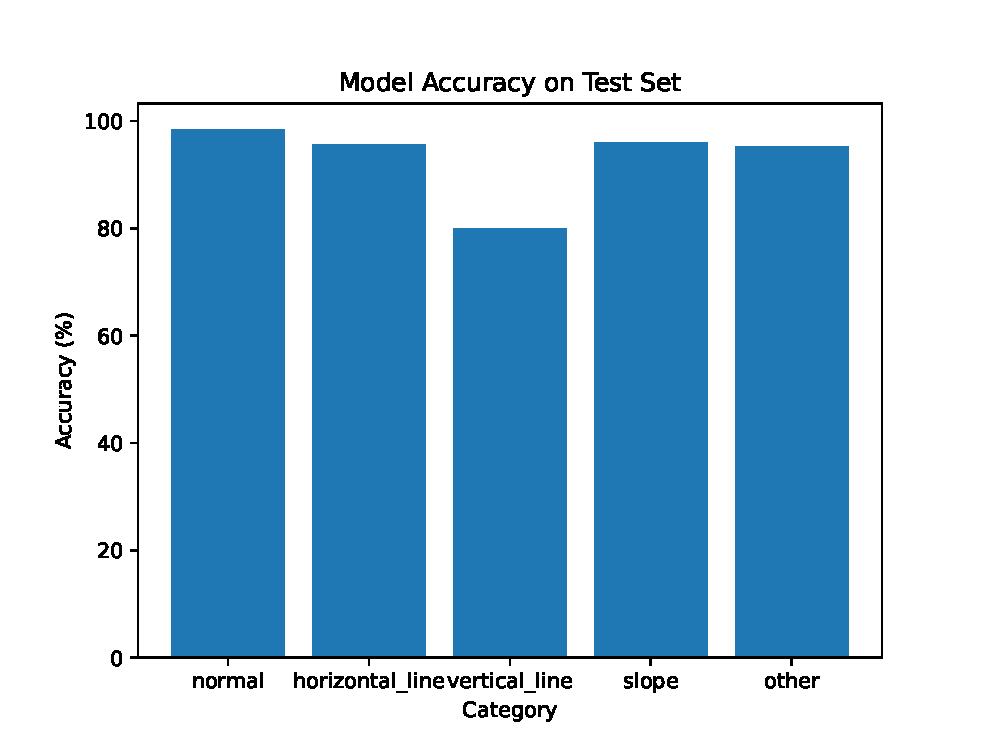
\includegraphics[width=\textwidth]{./fig/assistplot/accuracy.eps}
        \captionof{figure}{Accuracy on Test Set}
        \label{fig:accuracy_histogram}
    \end{minipage}
\end{figure}


\textbf{模型性能分析}

模型在"正常"类别中的表现非常出色,准确率达到98.4%,这表明它在识别没有明显缺陷的组织切片方面具有强大的能力。同样,"水平线"和"其他"类别的准确度也很高,反映出模型在识别这些特定类型的缺陷方面的有效性。

然而,"垂直线"类别的准确度明显较低,只有80.0%。这表明模型识别这种类型缺陷的能力需要加强。这可能是由于训练数据不足,限制了模型的学习。也可能是因为垂直线的特征相对不太明显,使得模型难以准确提取特征。

\subsection{模型的改进(改变输入分辨率)}

在这里,我们将讨论模型进一步改进的可能性。

将高分辨率图像缩放到InceptionV3模型所需的默认大小299x299,确实可能导致信息和细节的丢失。这对于原始分辨率较高的图像尤其关键,例如VHX7000设备拍摄的2880x2160的图像。直接缩小这些图像可能会阻碍模型捕获所有微妙差异的能力,这在医学成像等细节丰富至关重要的领域尤其有害。

一种可能的解决方案是修改模型的输入层,以接受更大的图像尺寸。这种方法使模型能够处理更高分辨率的图像,从而保留更多的原始信息和细节,这可能会提高性能和准确度。InceptionV3架构,其具有多个不同核大小的卷积,特别适合处理更大的图像,因为它可以有效地捕获不同尺度的特征。

由于实验室硬件(16GB的显存)的限制,图像被缩放到原始大小的0.4倍,因此在这个实验中,图像的尺寸为1152x864。

\textbf{Training the New Model (Model 4)}

Model 4 is trained with these adjusted image sizes, and its training effectiveness is as follows:

\begin{figure}[H]
    \centering
    \begin{minipage}{0.45\textwidth}
        \centering
        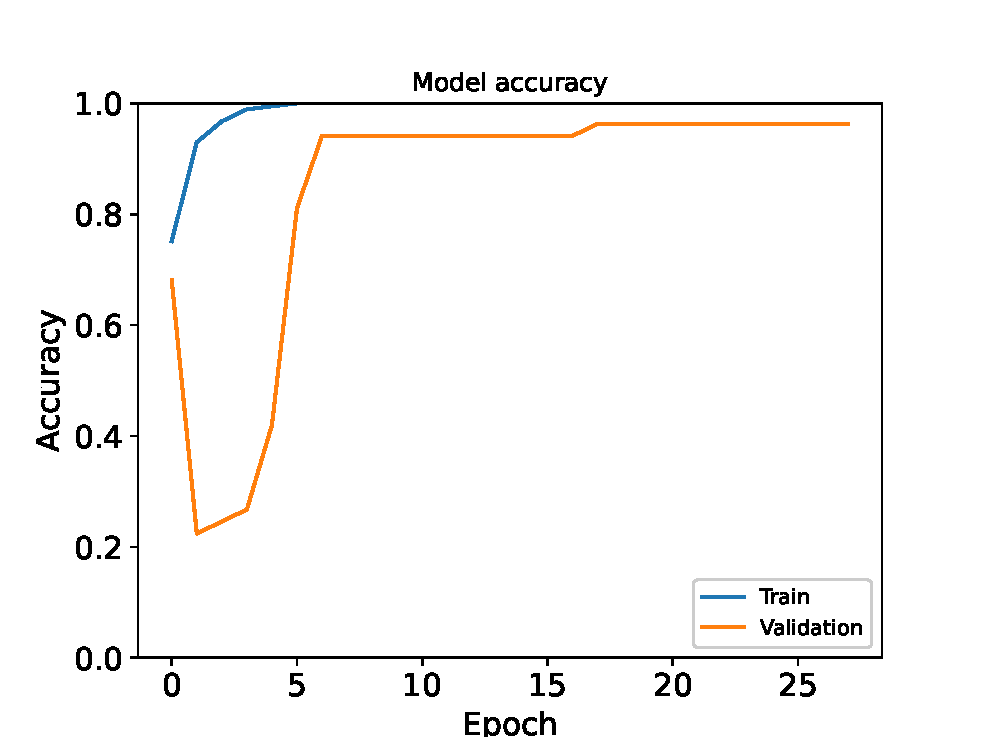
\includegraphics[width=\textwidth]{./fig/model4/accuracy4.eps}
        \caption{Model-4 accuracy}
        \label{fig:model4_accuracy}
    \end{minipage}
    \begin{minipage}{0.45\textwidth}
        \centering
        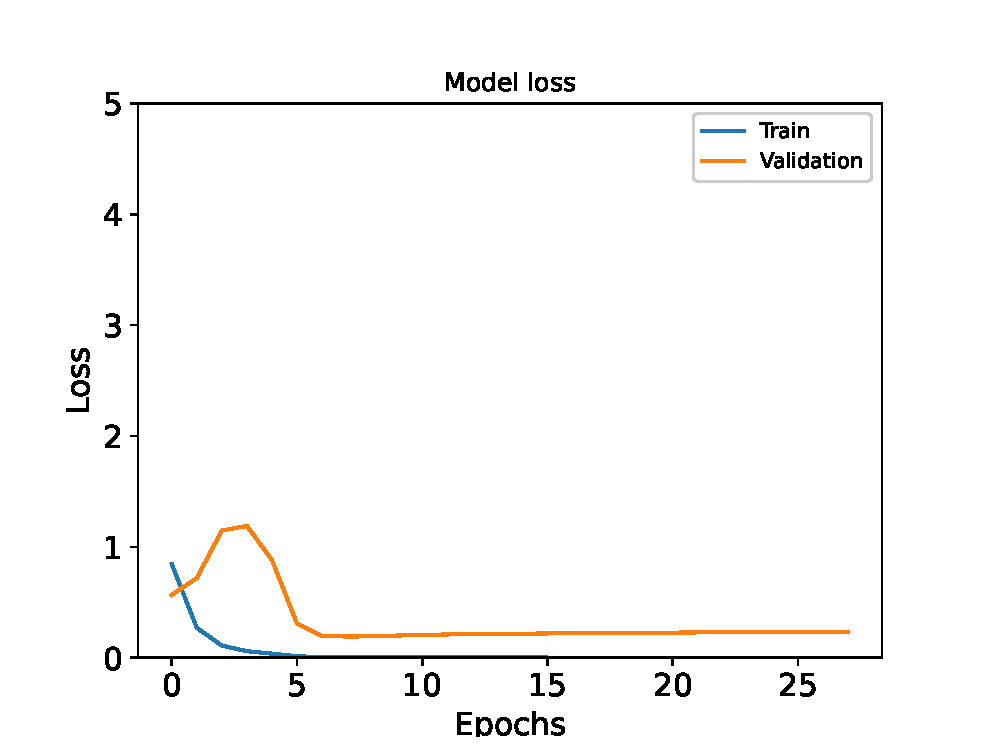
\includegraphics[width=\textwidth]{./fig/model4/loss4.eps}
        \caption{Model-4 loss}
        \label{fig:model4_loss}
    \end{minipage}
\end{figure}

通过观察训练准确性和损失随时间的变化,我们可以看到模型性能有了显著的提升。训练和验证的准确性都接近1,验证损失降低到大约0.2,这表明模型具有强大的泛化能力。这表明模型不仅在训练数据上表现优秀,而且能够有效地泛化到新的、未见过的数据。

\textbf{在测试集上重新评估准确性}

更新后的模型然后在测试集上重新进行评估,结果如\autoref{tab:model_accuracy2}所示:

\begin{table}[H]
    \centering
    \caption{model accuracy on test set}
    \begin{tabular}{cccccc}
        \toprule
        & normal & horizental\_line & vertical\_line & slope & other \\
        \midrule
        accuracy(\%) & 98.4 & 96.7 & 85.6 & 96.5 & 96.5 \\
        \bottomrule
    \end{tabular}
    \label{tab:model_accuracy2}
    \end{table}

比较改变分辨率前后的准确性,有明显的提升,尽管不是很大。这种适度的增加可能归因于已经接近1的高准确性,进一步的改进有递减的回报。

结果证实了处理高分辨率图像的潜在好处,特别是在需要高保真和细节的设置中,如生物组织分析和研究。

\subsection{研究机器的最佳切割角度}

为了确定微切机的最佳切割角度,我们准备了在8到12度之间,以0.5度为增量的各种角度切割的组织切片图像。每个角度类别包含100个图像,总共有9个不同的数据组。然后使用模型4来评估每组的质量率,目标是找出获得高质量切片最多的角度。

下表和图形展示了每个切割角度的准确性,定义为高质量切割的百分比:

\begin{figure}[H]
    \centering
    \begin{minipage}{0.4\textwidth}
        \centering
        \captionof{table}{Normal accuracy on different angle}
        \begin{tabular}{cc}
            \toprule
            Angle & Accuracy(\%) \\
            \midrule
            8 & 80 \\
            8.5 & 81.5 \\
            9 & 83.5 \\
            9.5 & 93.3 \\
            10 & 96.6 \\
            10.5 & 88.8 \\
            11 & 84.2 \\
            11.5 & 66.6 \\
            12 & 62.2 \\
            \bottomrule
        \end{tabular}
        \label{tab:model_accuracy_angle}
    \end{minipage}
    \begin{minipage}{0.55\textwidth}
        \centering
        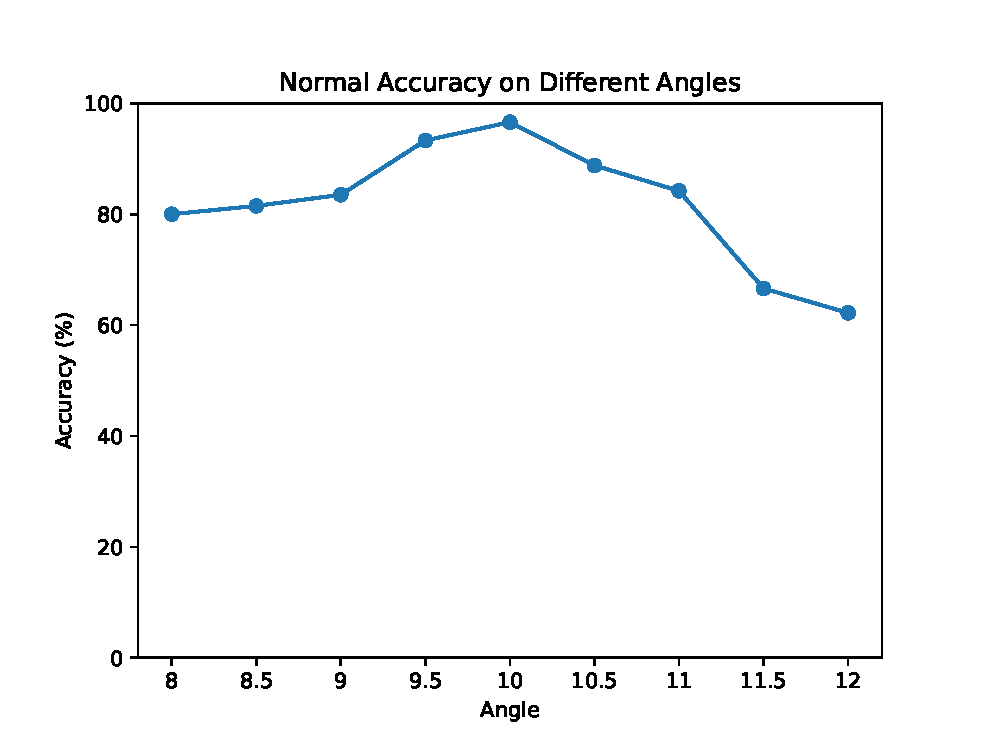
\includegraphics[width=\textwidth]{./fig/assistplot/angle_accuracy.eps}
        \captionof{figure}{Model Accuracy on Different Angle}
        \label{fig:angle_accuracy_histogram}
    \end{minipage}
\end{figure}

从\autoref{tab:model_accuracy_angle}中的数据可以看出,获得最高质量组织切片的最佳切割角度是10度,准确性高达96.6%。

此外,如\autoref{fig:angle_accuracy_histogram}所示,为了保持至少80%的切片质量率,切割角度应设置在9到10.5度之间。这个范围不仅确保了高质量切割的比率,而且还提供了一些机器设置的灵活性,以适应可能的组织类型或条件的变化。

\subsection{模型的泛化性}

到目前为止,实验已经使用了来自鱼类的卵巢组织切片。在实际应用中,我们可能会遇到各种各样的组织样本,包括其他器官或来自不同动物的标本。因此,评估我们的模型在各种组织类型上的泛化能力是至关重要的。

我们已经准备了一个新的数据集,包括鱼类肺部组织切片,分为四类:好、正常、差和其他。这些类别在下面的图中展示:(如\autoref{fig:fish_lung})

\begin{figure}[H]
    \centering
    \begin{minipage}{0.24\textwidth}
        \centering
        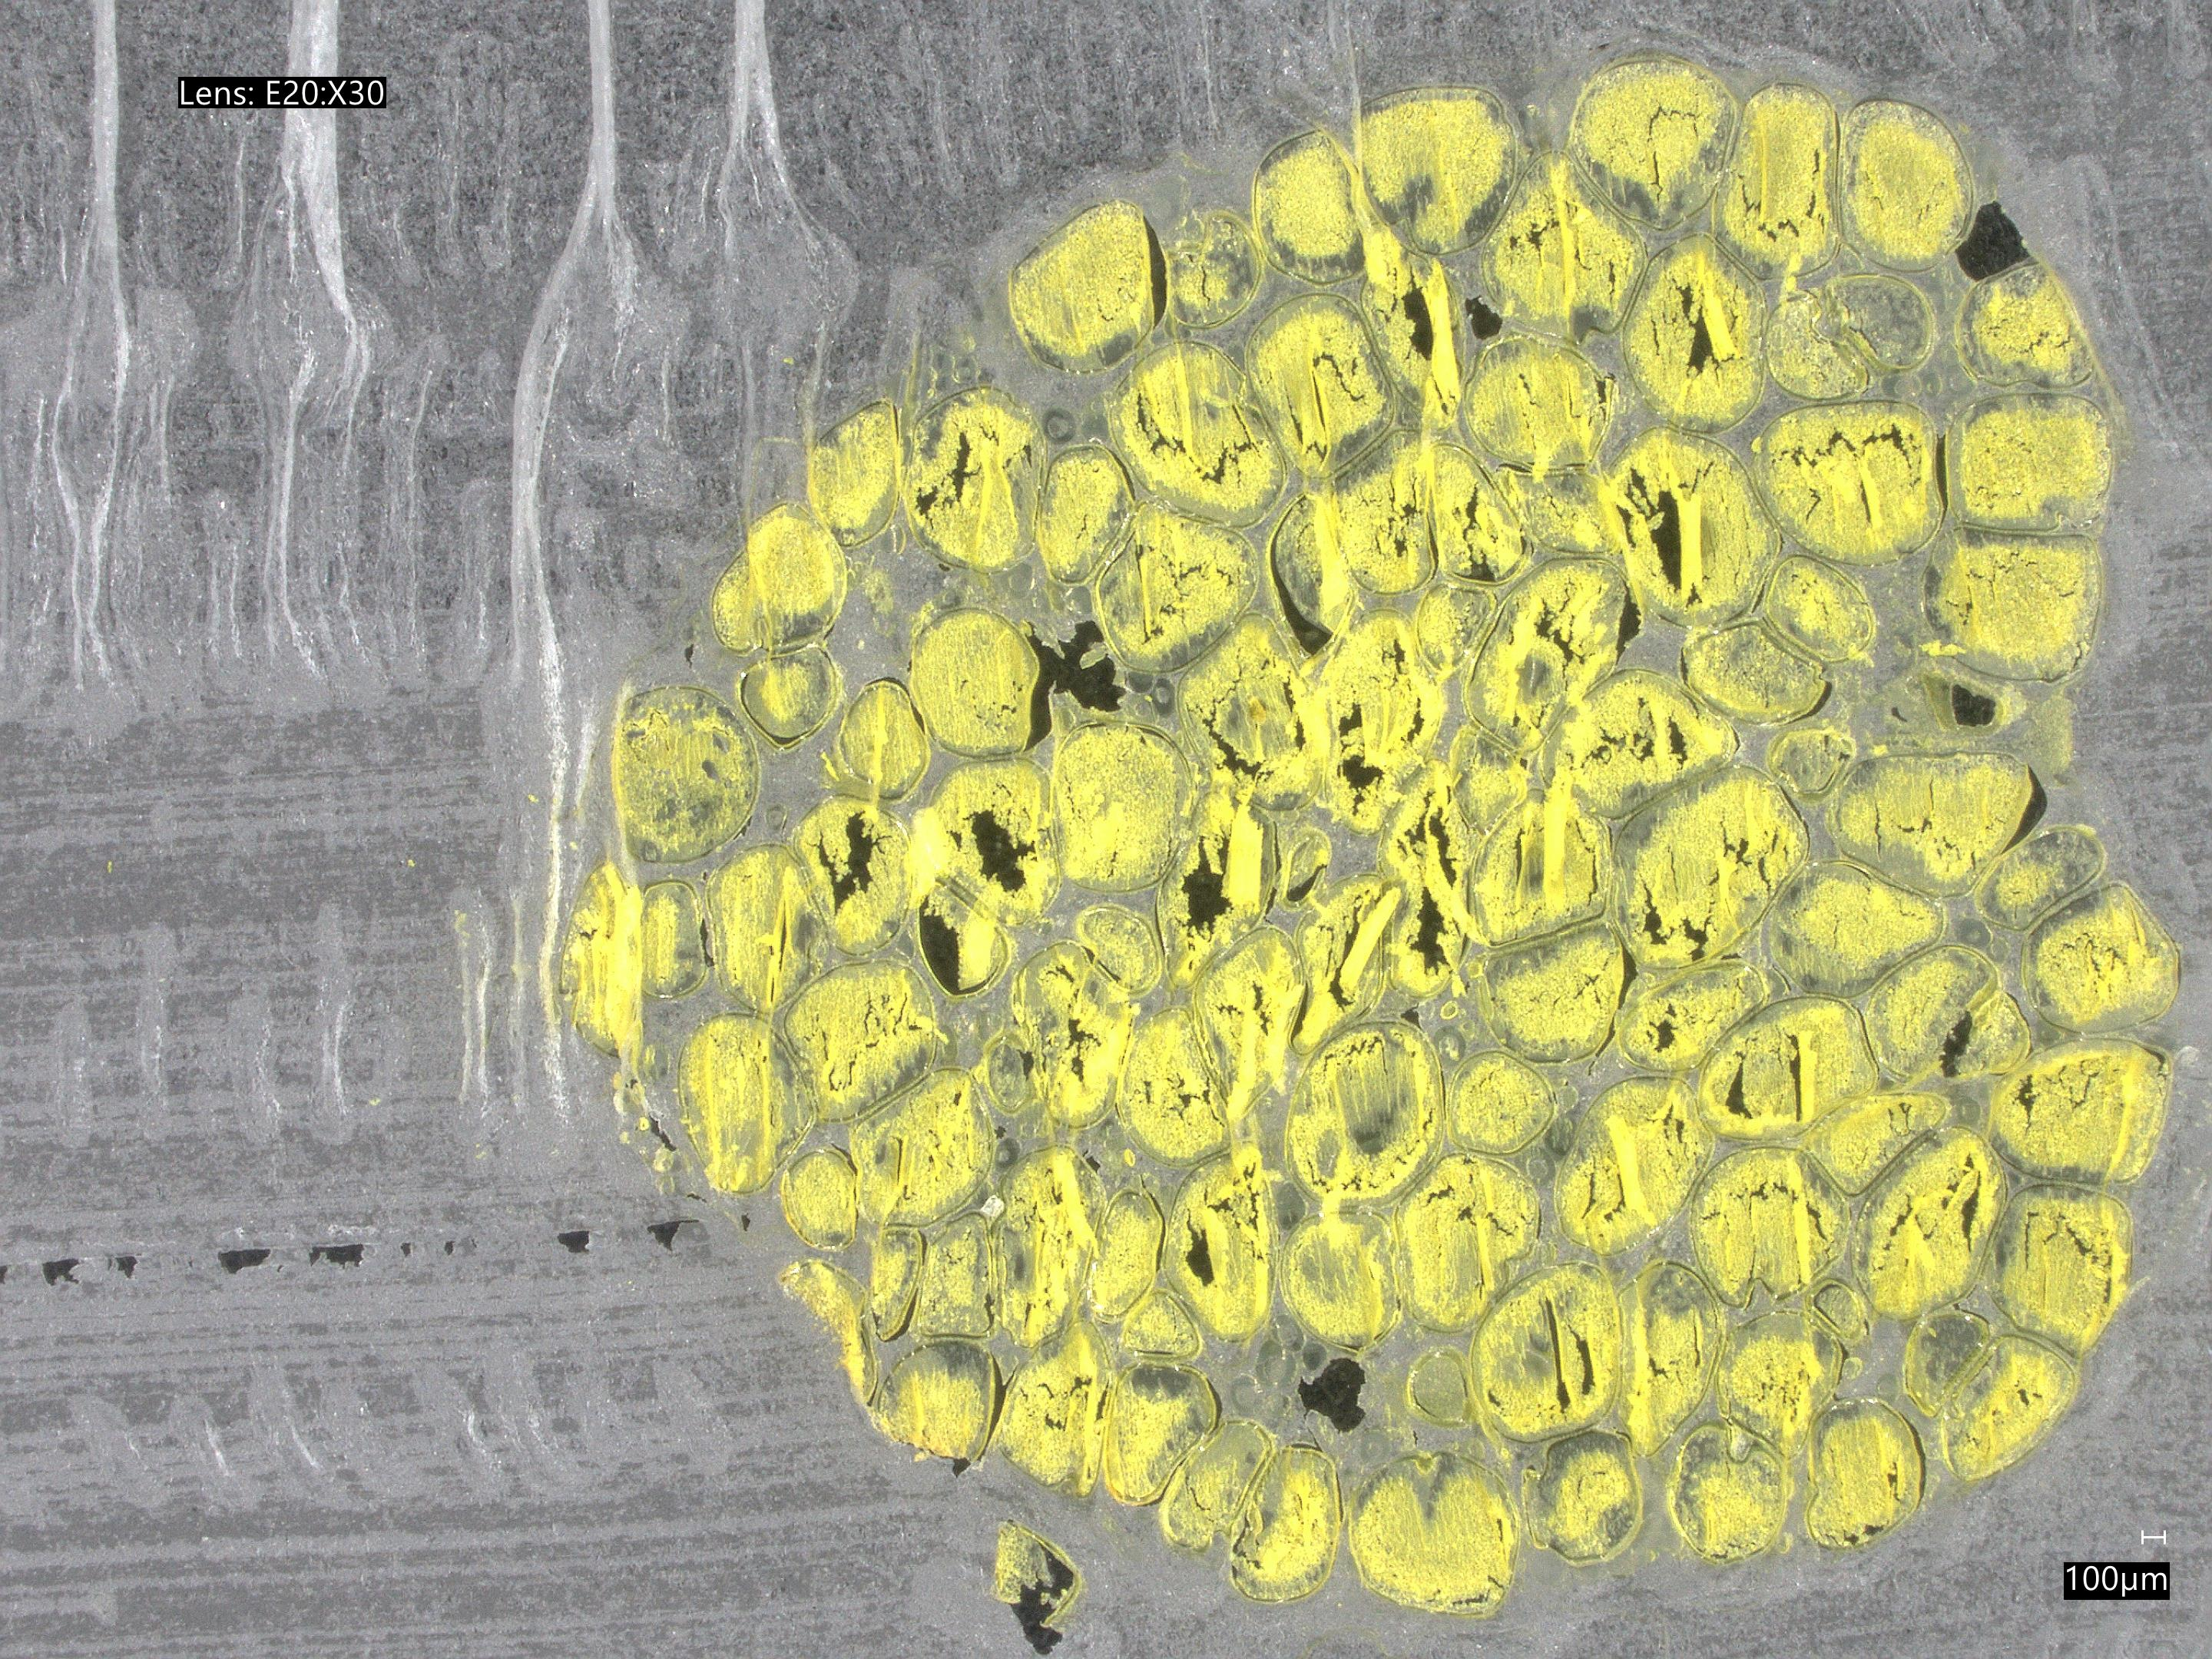
\includegraphics[width=\textwidth]{./fig/fish_lung/good20240313_144138.jpg}
        \caption*{Good}
        % \label{fig:good_fish_lung}
    \end{minipage}
    \begin{minipage}{0.24\textwidth}
        \centering
        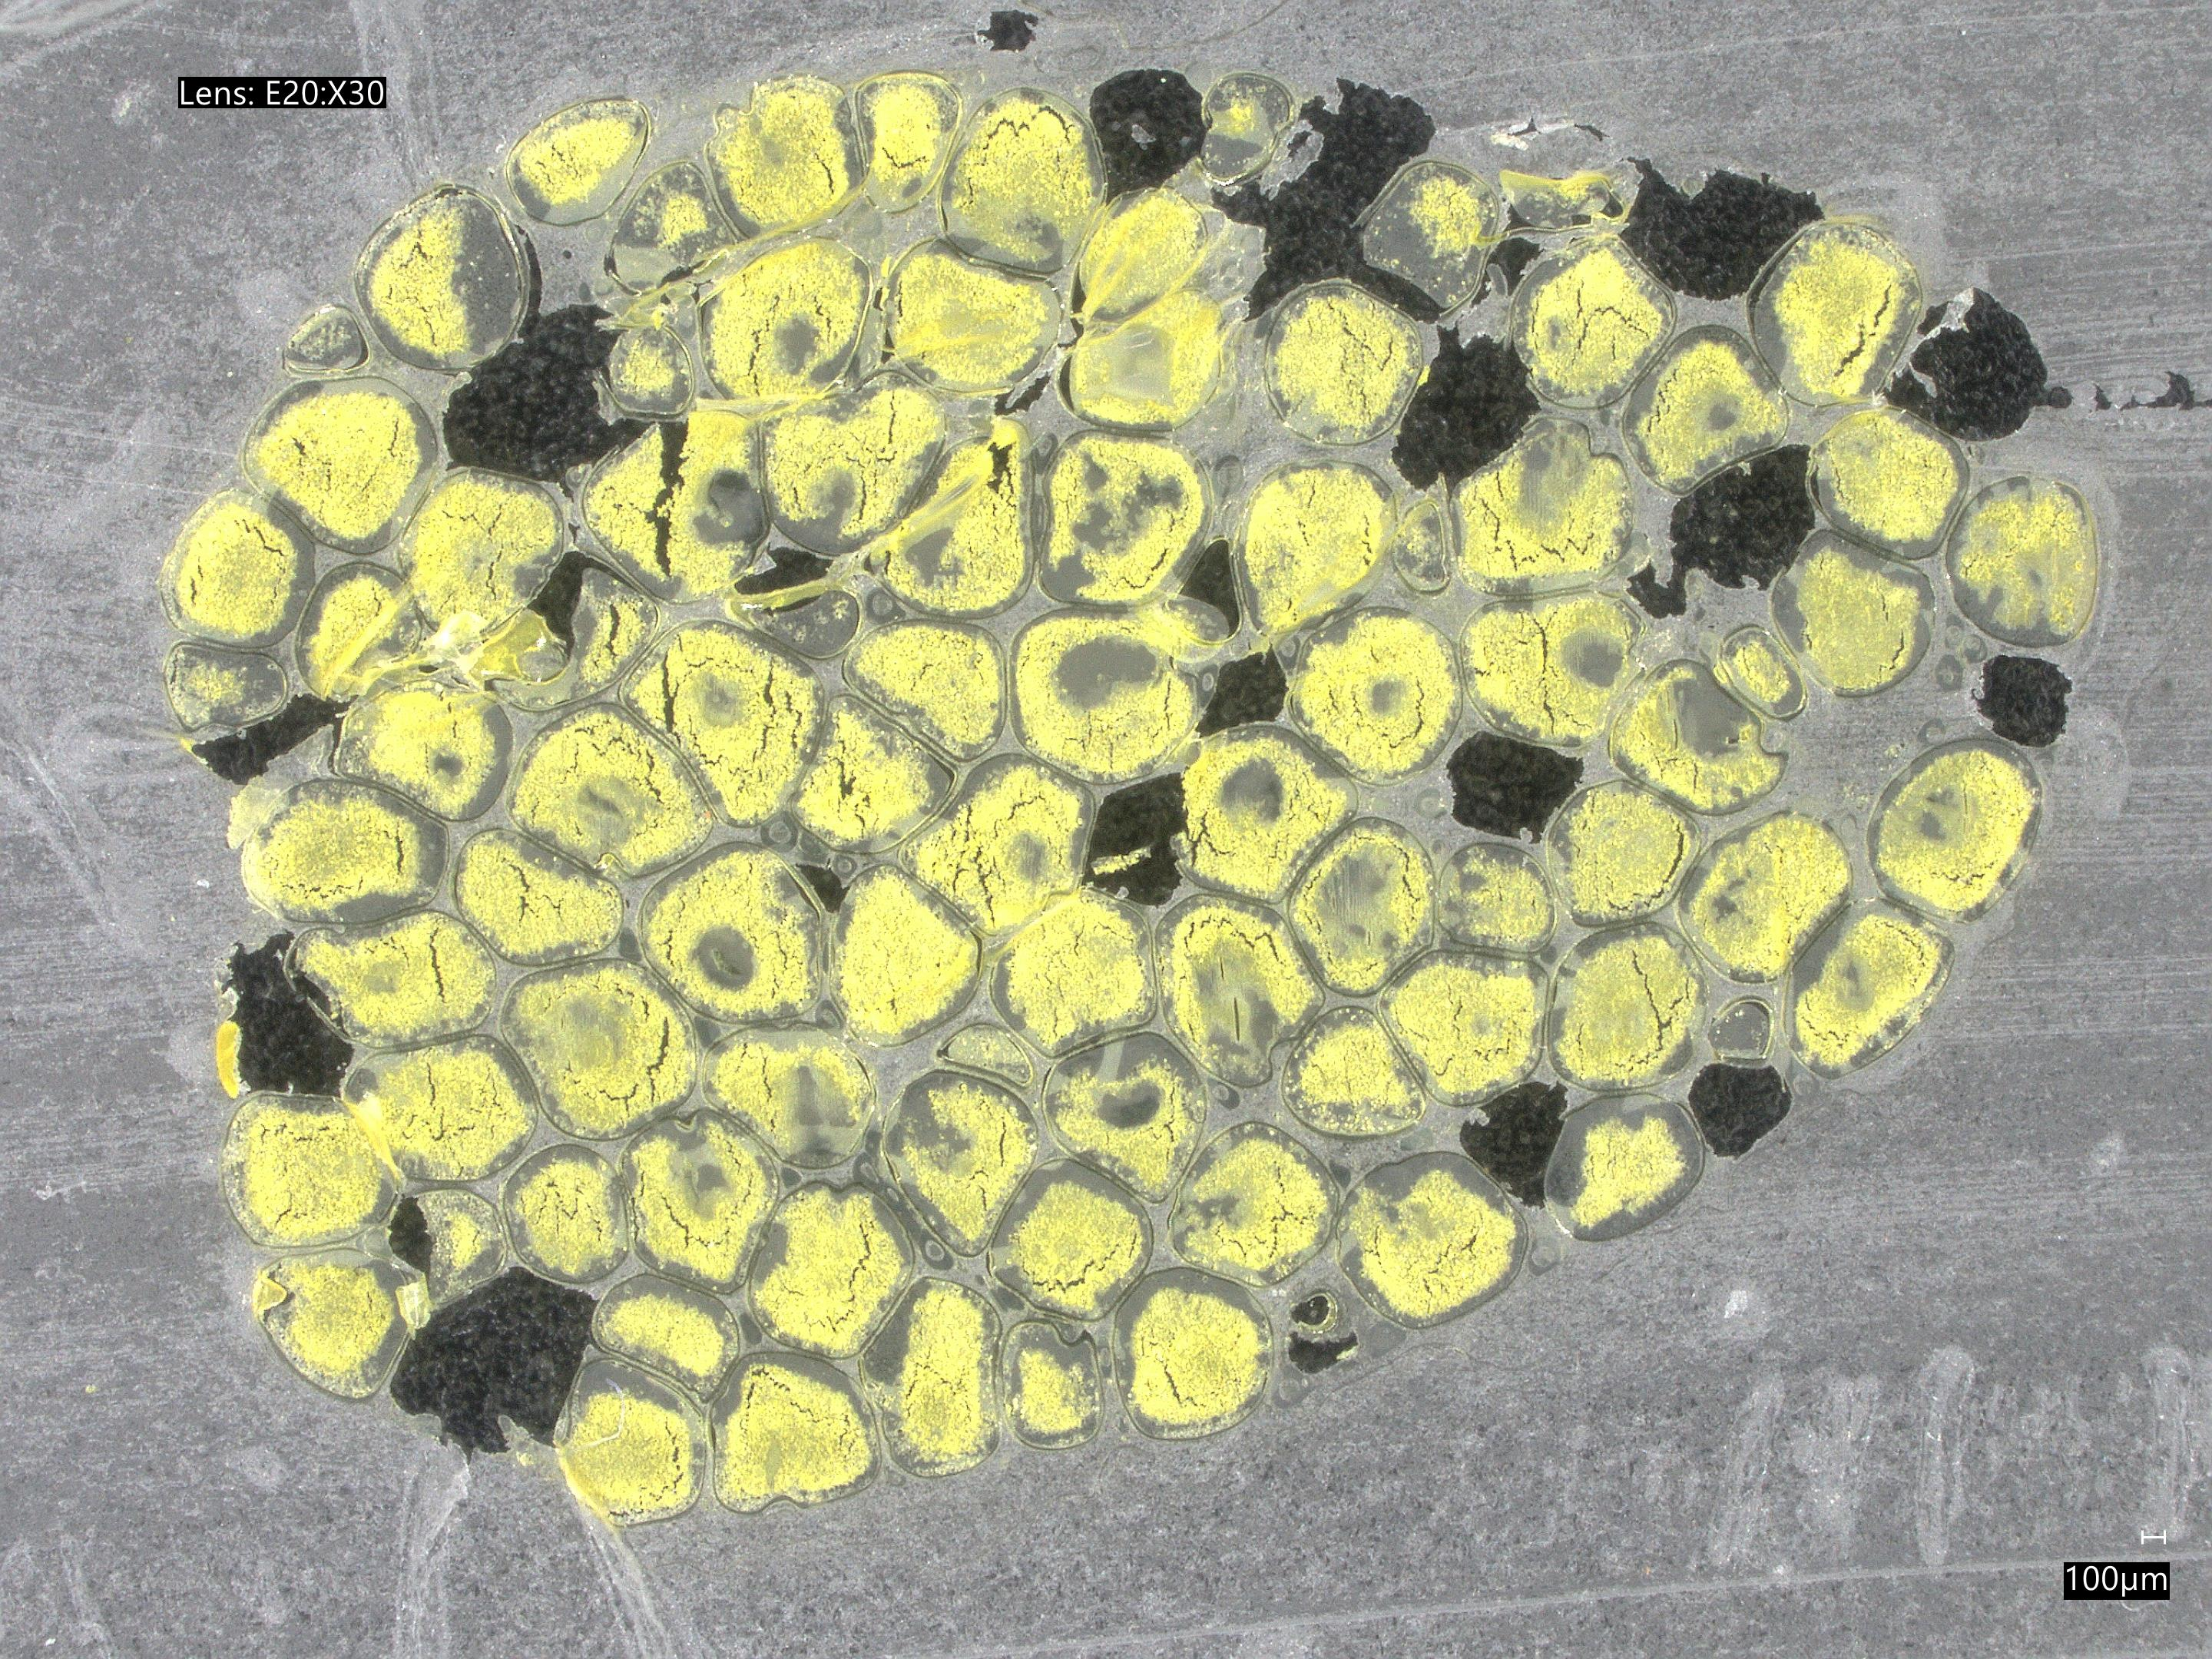
\includegraphics[width=\textwidth]{./fig/fish_lung/normal20240313_141726.jpg}
        \caption*{Normal}
        % \label{fig:noraml_fish_lung}
    \end{minipage}
    \begin{minipage}{0.24\textwidth}
        \centering
        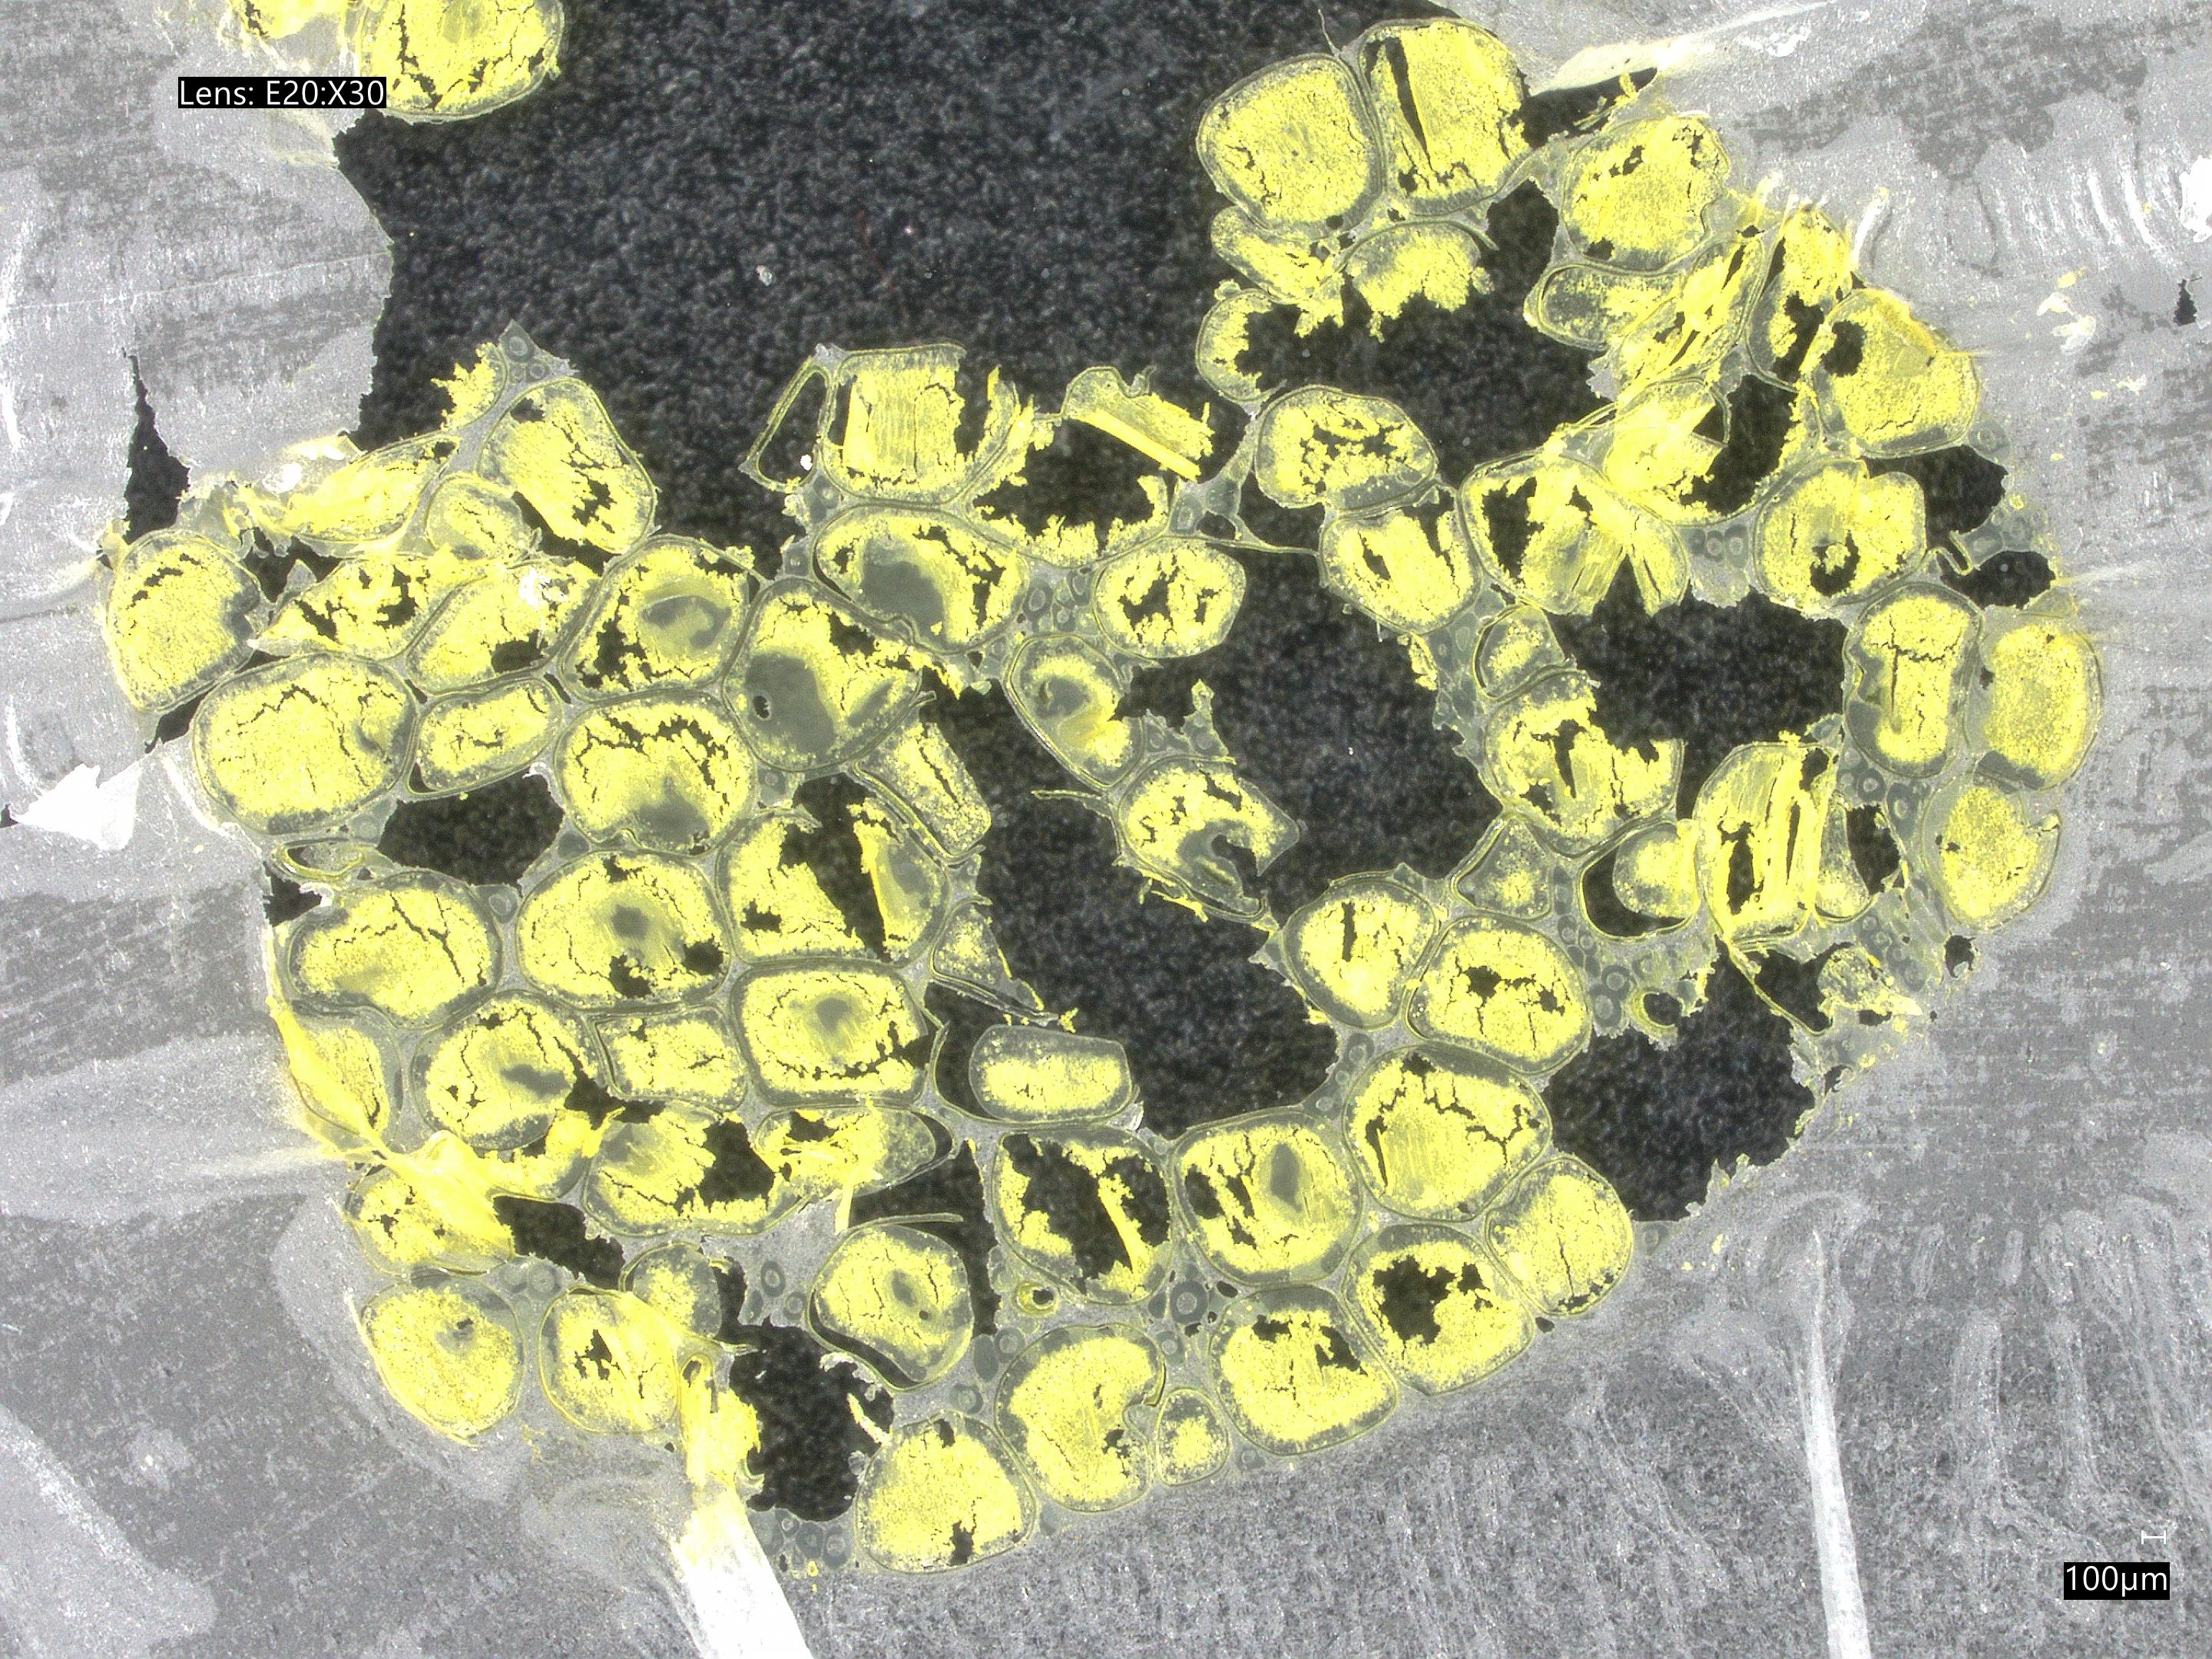
\includegraphics[width=\textwidth]{./fig/fish_lung/bad20240313_140952.jpg}
        \caption*{Bad}
        % \label{fig:bad_fish_lung}
    \end{minipage}
    \begin{minipage}{0.24\textwidth}
        \centering
        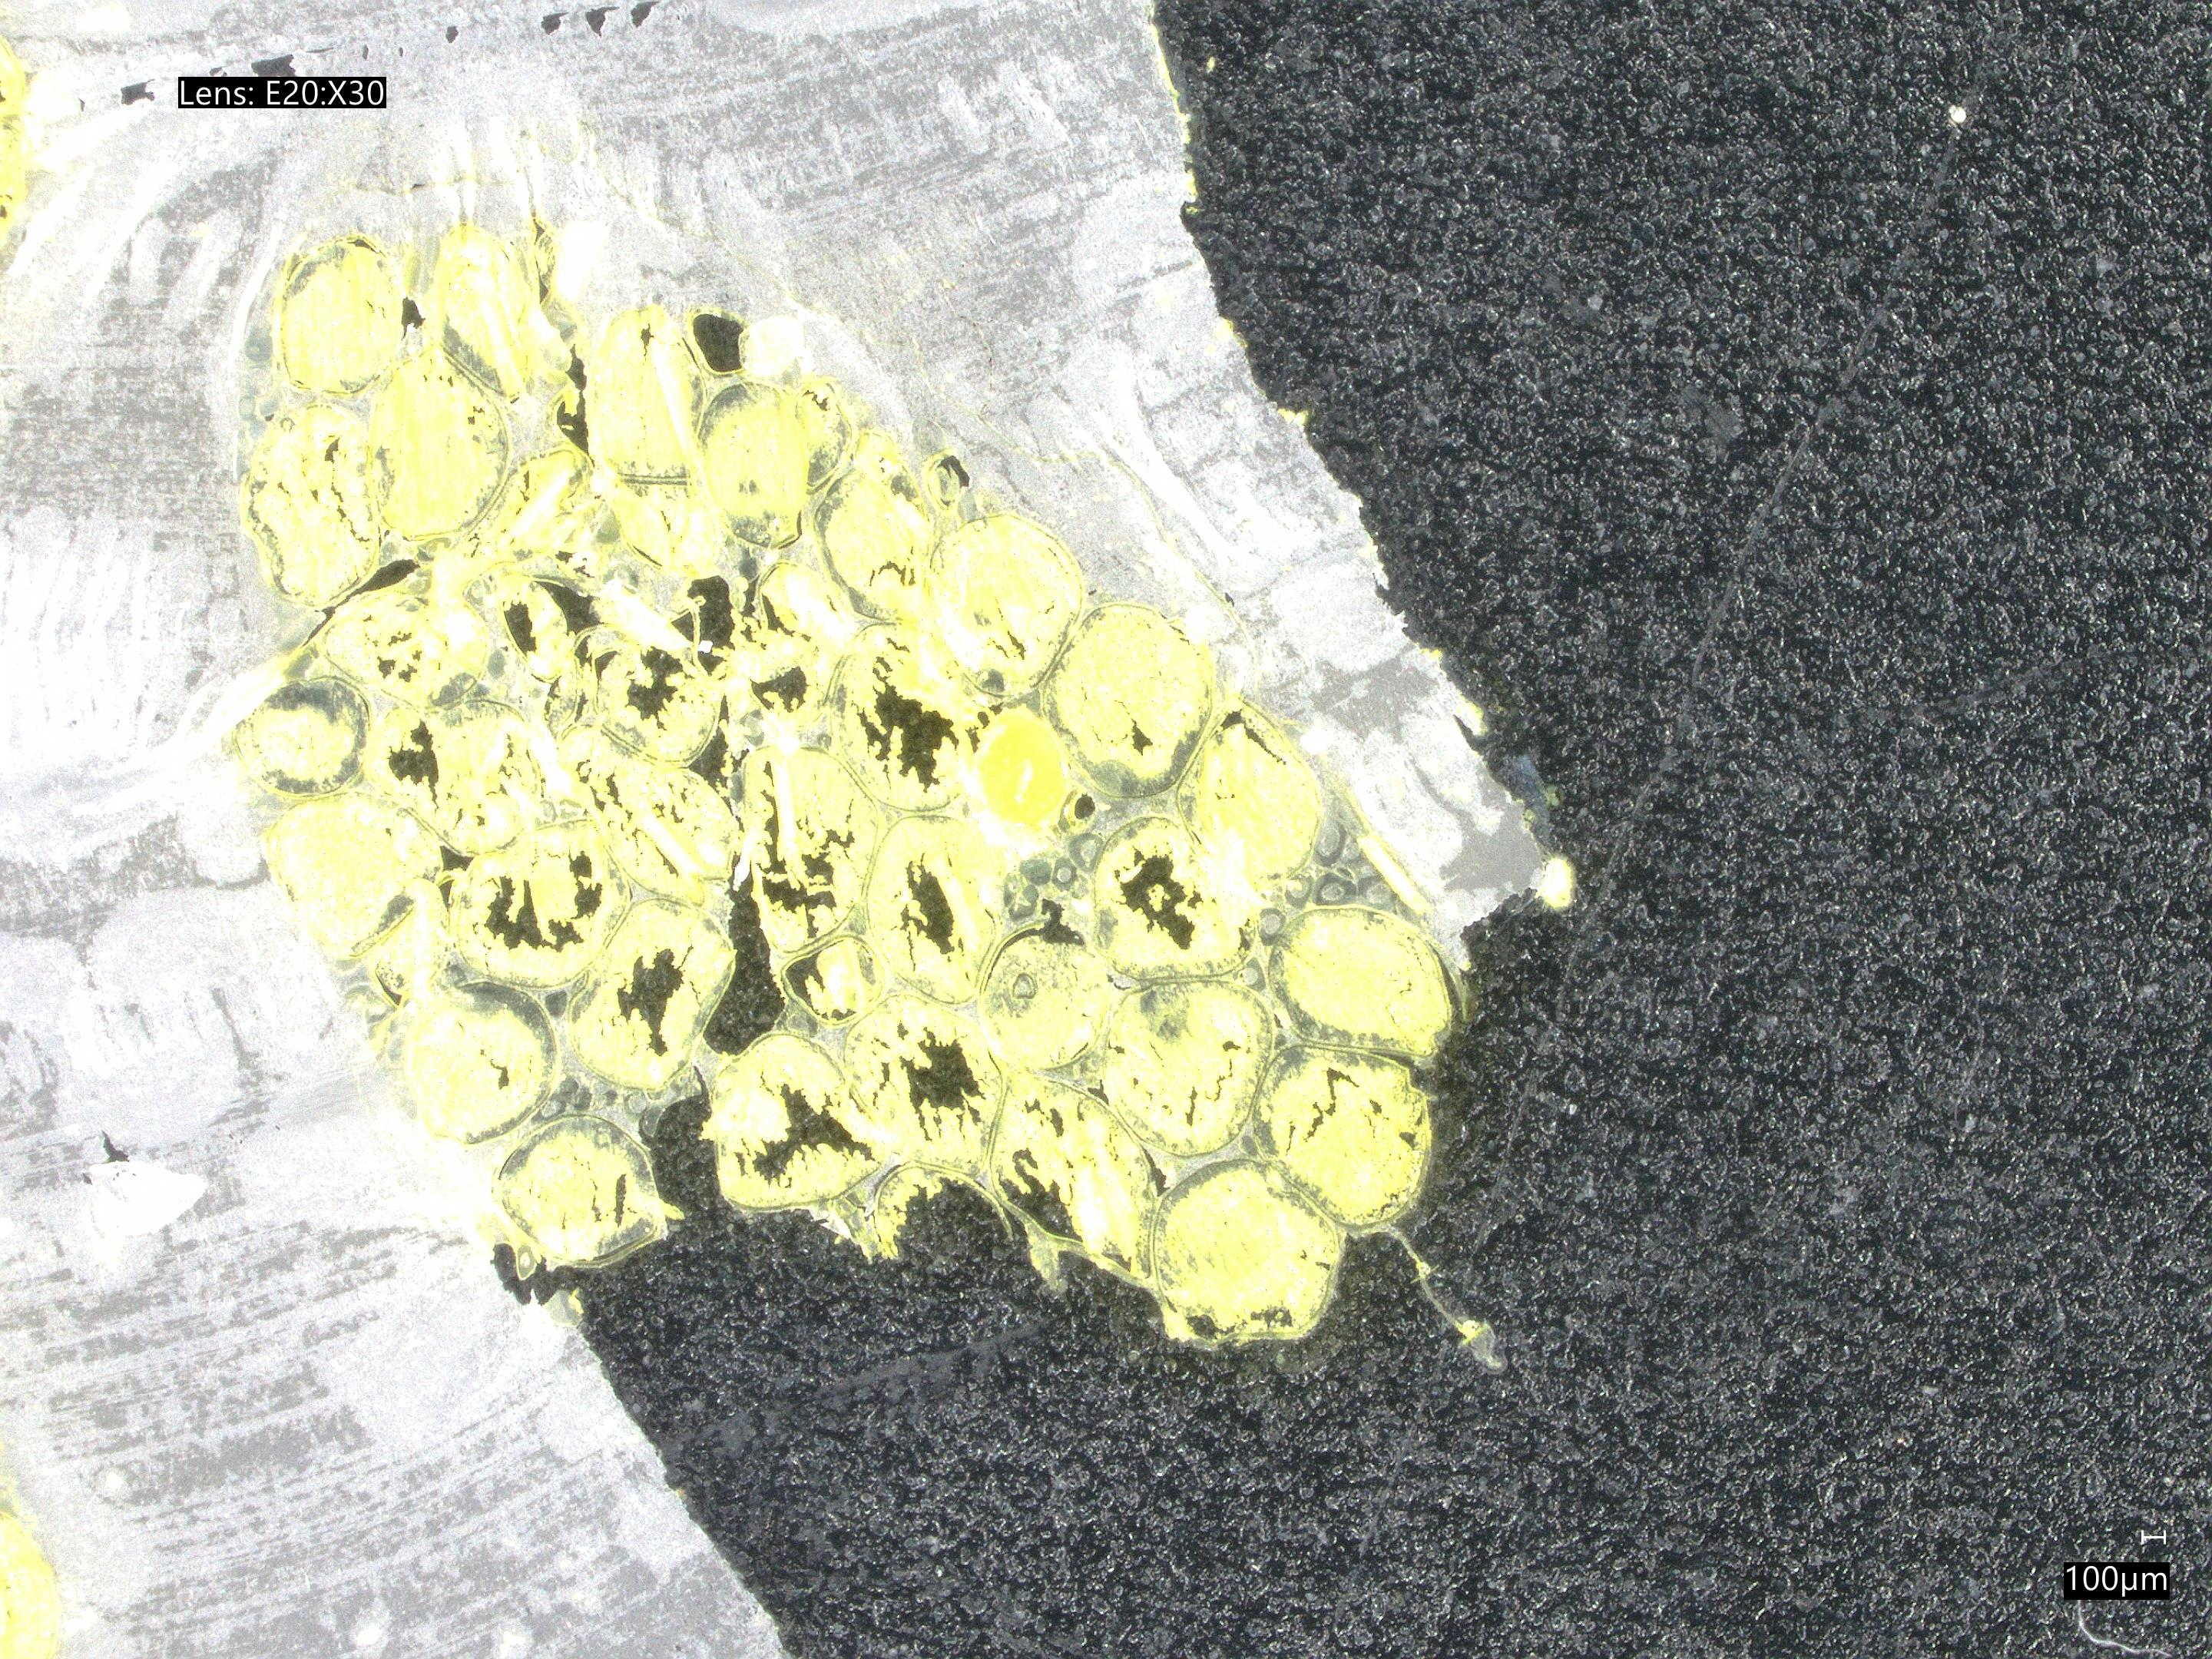
\includegraphics[width=\textwidth]{./fig/fish_lung/other20240313_141858.jpg}
        \caption*{Other}
        % \label{fig:other_fish_lung}
    \end{minipage}
    \caption{Four categories of fish lung tissue}
    \label{fig:fish_lung}
\end{figure}

保持原始的模型架构(模型4),但使用分辨率为1152x864的鱼肺图像重新训练。训练的准确性和损失在\autoref{fig:model5_acc}和\autoref{fig:model5_loss}中展示。
\begin{figure}[H]
    \centering
    \begin{minipage}{0.45\textwidth}
        \centering
        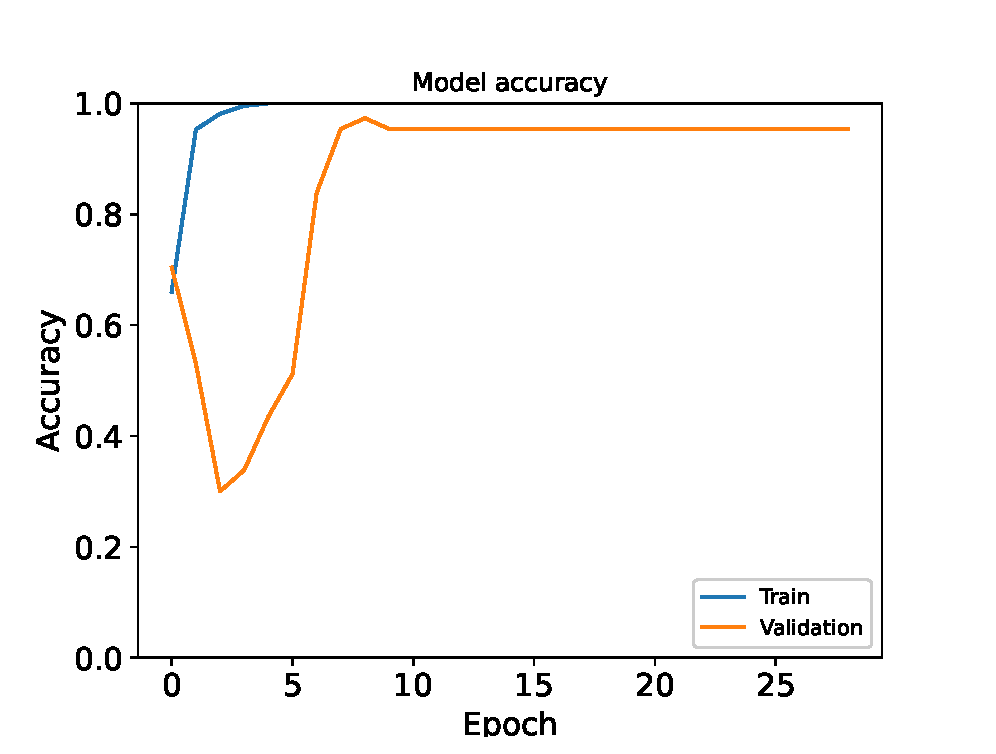
\includegraphics[width=\textwidth]{./fig/fish_lung/accuracy5.eps}
        \caption{Model-5 accuracy}
        \label{fig:model5_acc}
    \end{minipage}
    \begin{minipage}{0.45\textwidth}
        \centering
        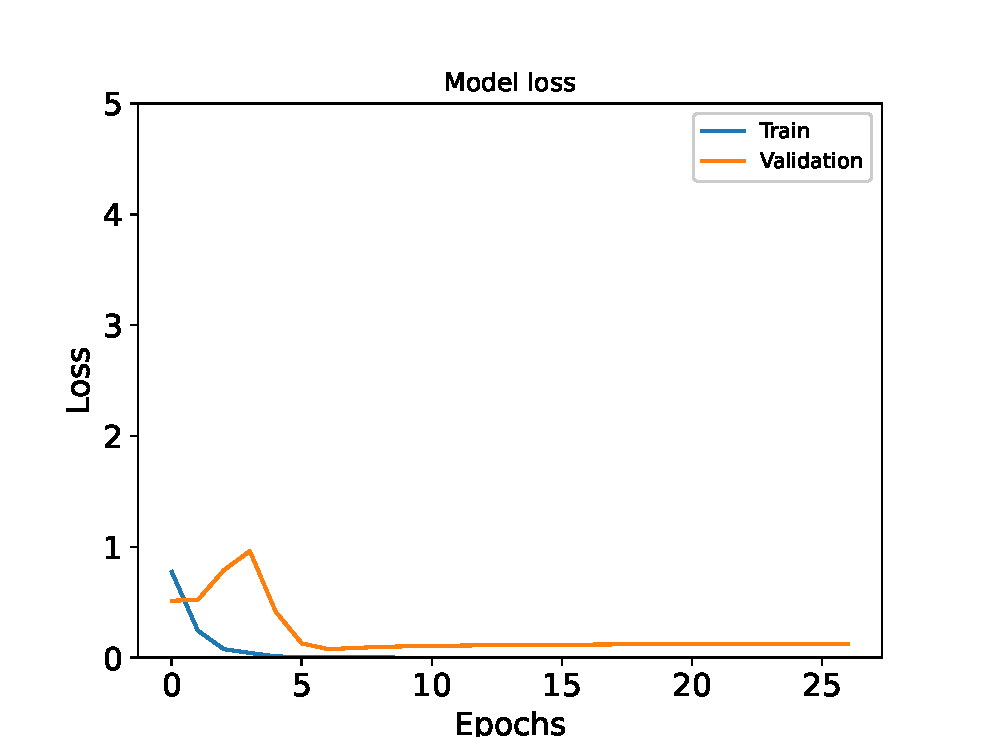
\includegraphics[width=\textwidth]{./fig/fish_lung/loss5.eps}
        \caption{Model-5 loss}
        \label{fig:model5_loss}
    \end{minipage}
\end{figure}

训练和验证的准确性迅速增加并保持在高水平,表明模型在两个数据集上的性能都很强。损失图显示训练损失迅速下降到零,验证损失在初期的激增后稳定下来,这表明模型的拟合和泛化性都很好。

模型进一步在测试集上进行测试,结果显示在\autoref{fig:accuracy_histogram2}中。

\begin{figure}[H]
    \begin{minipage}{0.45\textwidth}
        \centering
        \captionof{table}{Model accuracy on test set}
        \begin{tabular}{ccccc}
            \toprule
            label & accuracy(\%) \\
            \midrule
            bad & 94.1 \\
            good & 98.2 \\
            normal & 94.7 \\
            other & 95.0 \\
            \bottomrule
        \end{tabular}
        \label{tab:model_accuracy3}
    \end{minipage}
    \begin{minipage}{0.45\textwidth}
        \centering
        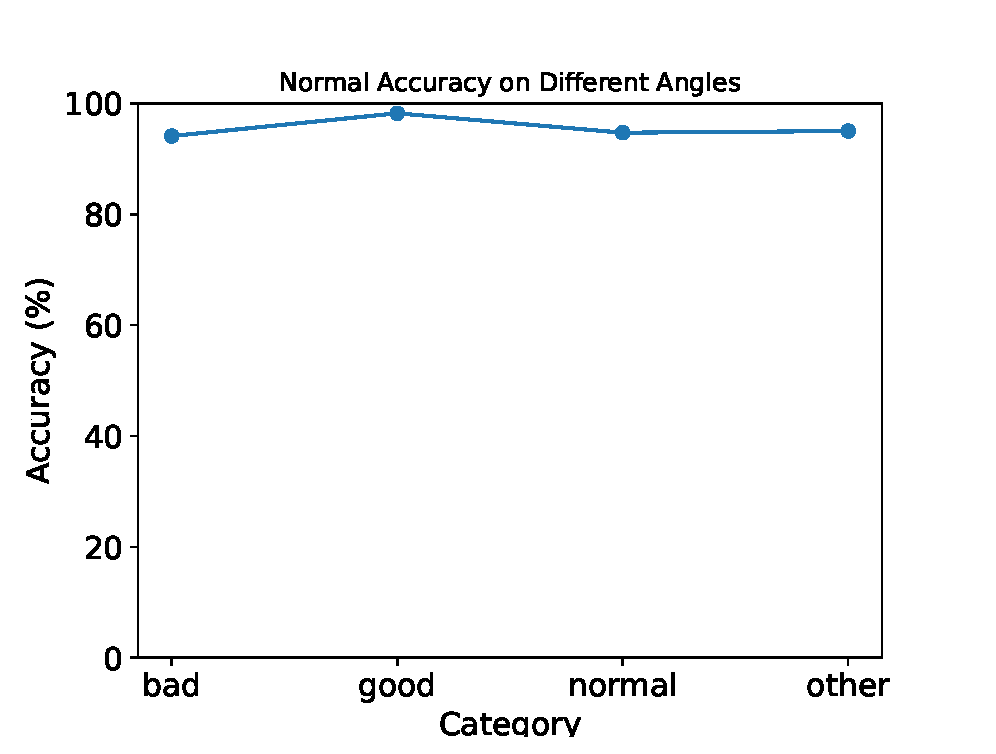
\includegraphics[width=\textwidth]{./fig/assistplot/angle_accuracy2.eps}
        \caption{Accuracy on Test Set}
        \label{fig:accuracy_histogram2}
    \end{minipage}
\end{figure}

该模型在所有标签上的准确率超过90\%,表明其强大的性能和显著的泛化能力。这表明该模型可以有效地分类不同类型的组织切片,可能使其成为各种生物医学成像应用的多功能工具。 模型在不同组织类型上的稳健性强调了其在组织质量评估和分类任务中的潜力。

\FloatBarrier
%result
\section{Discussion and conclusions}
\label{sec:results}

\subsection{Discussion of results}


% 如上所述,这项研究旨在建立一个可靠的模型来分类组织切片图像。最初,我们实现了简单的CNN模型,但在观察到有限的成功后,研究转向了图像预处理,并最终确定了使用InceptionV3模型进行迁移学习,这产生了最好的结果。

% 值得注意的是,随着不同模型的试验,随着模型参数的调整或模型架构变得更复杂(如InceptionV3),模型的性能显著提高,即验证集的准确率变得更高,损失变得更低。

% 此外,比较模型系列1和2,我们发现使用预处理的图像来协助机器提取特征在图像分类任务中并不十分有效。图像处理可能导致重要细节和信息的丢失,从而影响机器的特征提取,进而影响模型的准确性和性能。

% 在第5节中,我们测试了模型的应用。首先,我们选择了一个额外的测试集来测试模型的准确性,并发现模型在所有测试集上的准确性都超过85\%。然后我们使用模型评估不同的切割角度,发现如果要保证切割质量在80\%以上,切割角度应在9度到10.5度之间。最后,我们使用了另一个鱼鳃切片图像的数据集进行二次验证,发现模型对测试集标签的预测准确性都在90\%以上,反映出该模型可以很好地应用于其他数据集。

% 下面展示的最终选定的模型配置,突显了我们在有效整合InceptionV3架构到训练框架中所采取的结构化方法。

如上所述,本研究旨在建立一个可靠的用于分类组织切片图像的模型。最初,我们实现了简单的CNN模型,但在观察到有限的成功后,研究转向了图像预处理,并最终选择了与InceptionV3模型一起使用的迁移学习,这产生了最好的结果。

值得注意的是,随着不同模型的试验,随着模型参数的调整或模型架构变得更复杂(如InceptionV3),模型的性能显著提高,即验证集的准确率变得更高,损失变得更低。

此外,比较模型系列1和2,我们发现使用预处理的图像来协助机器提取特征在图像分类任务中并不十分有效。图像处理可能会导致重要细节和信息的丢失,从而影响机器的特征提取,进而影响模型的准确性和性能。

在第5节中,我们测试了模型的应用。首先,我们选择了一个额外的测试集来测试模型的准确性,发现模型在所有测试集上的准确性都超过了85\%。然后我们使用模型来评估不同的切割角度,发现如果要保证切割质量在80\%以上,切割角度应在9度到10.5度之间。最后,我们使用了另一个鱼鳃切片图像的数据集进行二次验证,发现模型对测试集标签的预测准确性都在90\%以上,反映出该模型可以很好地应用于其他数据集。

下面展示的最终选择的模型配置,突出了我们如何有效地在训练框架中整合InceptionV3架构的结构化方法。
% \begin{center}

%     \begin{tikzpicture}[node distance=1.5cm,
%         box/.style={
%             rectangle,
%             rounded corners,
%             draw=black, very thick,
%             text width=15em,
%             minimum height=2em,
%             text centered},
%         arrow/.style={
%             thick,
%             ->,
%             >=stealth}
%         ]
    
%         \node (collect) [box] {输入层:1152*864};
%         \node (mix) [box, below of=collect] {基础模型:InceptionV3};
%         \node (train) [box, below of=mix] {全局平均池化层};
%         \node (test) [box, below of=train] {全连接层(节点个数取决于标签)-输出层};
%         \node (evaluate) [box, below of=test] {学习率:1e-4,优化器:Adam};
%         \node (rate) [box, below of=evaluate] {损失函数:交叉熵,评估指标:准确率};
%         \node (improve) [box, below of=rate] {早停:启用};
        
%         \draw [arrow] (collect) -- (mix);
%         \draw [arrow] (mix) -- (train);
%         \draw [arrow] (train) -- (test);
%         \draw [arrow] (test) -- (evaluate);
%         \draw [arrow] (evaluate) -- (rate);
%         \draw [arrow] (rate) -- (improve);
        
%         \end{tikzpicture}
% \end{center}
\begin{itemize}
    \item Input Layer: 1152*864
    \item Base Model: InceptionV3
    \item Global Average Pooling Layer
    \item Fully Connected Layer (Number of nodes based on Labels) - Output Layer
    \item Learning Rate: 1e-4, Optimizer: Adam
    \item Loss Function: Cross-Entropy, Performance Metric: Accuracy
    \item Early Stopping: Enabled
\end{itemize}

\subsection{Future work}
\subsubsection{提升分类方法}

当前的研究表明,现有的分类方法具有前景,但仅限于五个类别。通过扩大这些类别,我们可以增强我们对切割角度如何影响样本质量的理解,并提高我们分析的精度。更广泛的分类范围也会更好地预测各种组织类型和条件的最佳切割角度。采用更详细的分类可以促进向线性分析方法的转变,其中增加的类别作为离散点,使得通过线性回归准确建模切割角度和样本质量之间的关系成为可能。

线性判别分析(LDA)对于改进我们如何确定与组织质量相关的最佳切割角度特别有用。这种方法可以简化切割参数的预测,并改善对组织切割的控制。然而,过渡到线性判别框架带来了挑战。与输出概率的二元模型不同,线性回归模型需要变量(如切割角度和组织质量)之间有直接的相关性,这可能并非固有的线性。

此外,线性模型需要大量的数据,这可能会延长数据收集的时间,增加其复杂性,并需要更多的计算能力。当前使用TensorFlow和InceptionV3的系统已经在压榨GPU资源,突显了需要增强硬件的需求。这些进步,对于有效使用线性判别分析至关重要,将需要大量的时间和资源,以及进一步的理论和实践研究。例如,Jie Wen在"Robust Sparse Linear Discriminant Analysis"的工作中,将稀疏性整合到LDA模型中,使其更加健壮,适合复杂的应用\cite{6.1}。

\subsubsection{探究其他参数对切削质量的影响}

在之前的实验中,我们把切削角度设置为自变量,切削质量设置为因变量,建立了一个模型。然而,实际上切削质量可能受到其他参数的影响,如切削速度、给进速度(切片厚度)、刀具磨损等。

在将来的工作中,如果我们重点研究切削质量的影响因素,那么关于其他变量的研究将会是必须的。事实上,关于这些参数对质量的影响可以用一个函数来直观的表示:

\begin{equation}
    Q = f(\theta, v, f, w)
\end{equation}

其中,Q代表切削质量,$\theta$代表切削角度,v代表切削速度,f代表给进速度,w代表刀具磨损。至于这个函数里面的具体形式,也就是各个参数所占的权重,则需要大量的实验数据来统计然后拟合。这又将是一个挑战。


\subsubsection{性能提升和优化}

随着这项研究向大规模应用进展,性能优化成为了一个关键的挑战。这不仅涉及提高算法效率,还包括改善模型框架的可扩展性、稳定性和部署能力,以及优化底层编程语言和代码。

为了优化计算资源的使用,采用更高效的计算框架和并行处理算法是必要的。利用分布式计算资源可以显著减少模型训练时间,并在处理大型数据集时提高效率。此外,考虑到能耗和计算成本的限制,优化模型的计算架构和参数设置以在有限资源内最大化输出是至关重要的。

文章"TensorFlow和PyTorch在卷积神经网络中的应用效率分析"强调了TensorFlow和PyTorch在处理卷积神经网络时的差异\cite{6.2}。TensorFlow展示了较低的错误率和较小的收敛步骤,而PyTorch提供了更快的训练速度。

Pascal Fua的"Comparing Python, Go, and C++ on the N-Queens Problem"通过比较Python、Go和C++在解决N皇后问题上的效率,提出了优化深度学习性能的方法。\cite{6.3}研究发现,运行时语言在处理循环和数据流方面有明显优势,这表明编译工具如Numba、Cython和Pybind11可以在深度学习应用中提高性能。

\subsubsection{切割过程的优化}

我们的研究还发现,在切割过程中实时评估切片质量,并根据这些评估进行调整,可以显著提高组织切片的质量。

我们提出的反馈调整过程包括在显微切片机上方安装一个摄像头,捕获正在切割的样本的数据。这些数据然后由预训练的模型实时分析,评估切片的质量。基于这个评估,可以调整显微切片机的切割速度和角度参数,以提高后续切片的质量,从而确保可控和一致的样本质量。

实施这个系统面临几个挑战:

\begin{itemize} \item \textbf{实时图像处理:}需要一个清晰的摄像头和一个高效的实时图像处理系统,以快速捕获和处理图像数据。 \item \textbf{强大的计算资源:}需要一个预训练的模型和一个强大的计算机,以快速评估图像并根据评估调整显微切片机的参数。 \item \textbf{有效的控制接口:}需要一个高效的控制接口,以确保调整后的参数能及时传达给显微切片机。 \item \textbf{时间效率:}整个系统必须在切割间隔内操作。 \end{itemize}

一个相关的例子可以在研究"Convolutional neural networks applied to microtomy: Identifying the trimming-end cutting routine on paraffin-embedded tissue blocks"\cite{6.4}中找到。这项研究通过用摄像头监控切割过程,用CNN分析图像,并根据分析调整显微切片机的参数,自动化了切割过程。显微切片机、摄像头和深度学习模型的集成为在切割过程中实时评估和调整切割参数提供了一种可行的解决方案。

\subsection{Conclusions}

% 这项研究通过将深度学习技术应用于生物医学组织切片设备,显著推进了我们对优化活检参数的理解。通过采用复杂的卷积神经网络,特别是通过转移学习对InceptionV3模型的改造,该研究展示了一个能够高精度评估组织切片质量的强大框架。这种方法不仅提高了组织样本分析的准确性,而且引入了组织切片操作方法的范式转变。

% 通过评估不同角度的切片质量,我们发现了切割角度和切片质量之间的关系。这为我们提供了一种在未来提高切片质量的可行方法。此外,该模型在不同类型的组织(包括鱼卵巢和肺组织)中的应用,证实了其广泛的适应性和推广潜力,表明它适合各种组织切片和研究任务。

% 然而,该研究也突出了传统图像预处理技术的局限性。初步尝试通过图像预处理来提高模型性能并没有带来显著的改进,而在某些情况下,可能会模糊掉进行准确分类所必需的关键细节。这个发现表明,保持原始图像数据的完整性可能比应用激进的预处理技术更有益。

% 研究还探讨了通过扩展分类方法和优化性能来增强组织切片过程。这包括将更多的分类类别和线性分析方法如线性判别分析(LDA)结合进来,从而更精确地理解切割参数与样本质量之间的关系。同时,通过采用更高效的计算框架和并行处理技术来优化性能,以及探索额外参数如切割速度和进给率,都将提升模型的预测能力和组织切片的质量。此外,实施实时反馈系统,利用机器学习动态调整切割参数,将推动组织学制备向自动化迈进,确保更一致和高质量的组织切片。

% 总的来说,这个项目不仅展示了深度学习在生物医学研究和应用中的重要作用,而且为进一步改进组织切割技术提供了可行性。这些技术的结合可以为生物切割设备带来改进,提供一种可能的解决方案来提高组织样本的产出率和切割效率。这项研究为未来的组织切割技术提供了新的思路和方法,预计将在生物医学领域产生深远影响。


本研究通过将深度学习与生物医学组织切片设备相结合,显著增强了对优化活检参数的理解。该研究采用了通过迁移学习调整的InceptionV3模型,展示了一个用于高精度评估组织切片质量的强大框架。这种创新方法不仅提高了组织分析的准确性,而且革新了组织切片的操作方法。

研究发现了切割角度与组织切片质量之间的明显相关性,提供了一种实用的方法来提高未来切片的质量。模型在各种组织类型(如鱼卵巢和肺组织)上的有效性,突显了其广泛的适应性和广泛应用的潜力。

然而,研究也指出了传统图像预处理技术的局限性。初步的预处理并没有显著提高性能,有时甚至模糊了准确分类所需的关键细节。这表明,保留原始图像数据可能比应用广泛的预处理更有利。

本研究通过扩展分类方法和性能优化,提出了对组织切割过程的改进。这包括整合更多的分类类别和线性分析方法,如线性判别分析(LDA),以精细化理解切割参数与样本质量之间的关系。此外,探索影响切割质量的其他因素也是至关重要的。未来的工作将专注于优化计算框架和并行处理,以及检查其他参数,如切割速度和进给速率,以提高模型的预测性和组织切片的质量。预计实施一个使用机器学习动态调整切割参数的实时反馈系统,将推动组织学准备向全自动化发展,确保始终高质量的组织切片。

总的来说,这个项目不仅强调了深度学习在推进生物医学研究和应用中的关键作用,而且为组织切片技术的大幅改进奠定了基础。这些进步可能会显著提高组织样本处理的产量和效率,为未来组织切片技术的发展提供新的策略和方法,对生物医学产生持久的影响。



\FloatBarrier % Now the table doesn't flow over to any other sections
%analyse
\section{Project management, consideration of sustainability and health and safety}

\label{sec:conclusion}
\subsection{Project management}

The primary tool for managing the project was a Gantt chart, as illustrated in \autoref{fig:gantt_chart}. This chart served as a visual tool to set and track realistic timelines for completing various sections of the project. It was updated throughout the project to reflect changes, including additions and deletions of project segments.

Regular updates to the chart, combined with weekly meetings with the supervisor, ensured the project remained on schedule.

% 管理项目的主要工具是甘特图,如图所示。这个图表作为一个可视化工具,用于设定和跟踪完成项目各个部分的实际时间表。在整个项目过程中,它会不断更新,以反映项目段落的增加和删除。

% 通过定期更新图表,并结合每周与导师的会议,确保了项目按计划进行。

\begin{figure}[htbp]
    \centering
    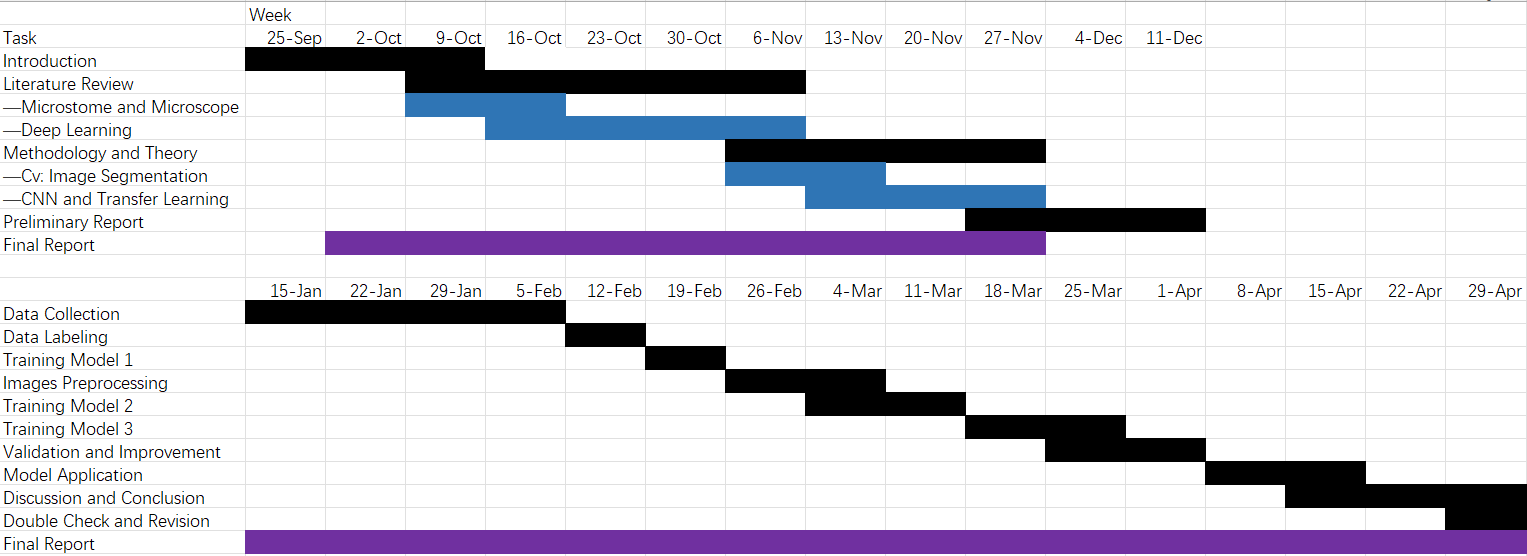
\includegraphics[width=1\textwidth]{./fig/gantt_chart.png}
    \caption{Gantt chart}
    \label{fig:gantt_chart}
\end{figure}


% \subsection{Health and safety}

% 在实验中唯一能产生安全风险的就是实验仪器的操作,其中主要风险是在制备生物切片和显微镜的操作。在制备切片是将会使用非常锋利的组织切片刀,因此在操作时需要特别小心,以免切到手指。我们在操作时严格遵守实验规范,戴上手套,避免直接接触刀片。此外,为了避免误伤和保证实验的一致性,在大部分情况下我们都使用机器的自动切削功能,而不是手动切削。这也就是说,在制备切片的过程中,实验人员仅仅负责对刀而剩下的事情都是由机器来完成的。

% 在显微镜采集图像时,主要风险是在调节显微镜时,不小心碰到显微镜的镜片,导致镜片破损。为了避免这种情况的发生,我们在操作时都尽量避免手工操作,而是通过显微镜的自动调节功能来调节焦距和光圈大小。这样能够避免在触摸转动显微镜头的同时污染镜头,导致成像质量的下降。

% \subsection{Sustainability}

% 有关于可持续性的考虑,在实验中的产物只有生物组织切片和玻璃片。对于这些已经使用的物品,我们严格按照垃圾分类的要求进行处理。对于生物组织切片,我们将其刮下并放入生物垃圾桶中,而对于玻璃片,特别考虑到其的锋利程度,我们需要将其进行简单包装后放入玻璃垃圾桶中。这样能够保证实验室的环境整洁,也能够保护实验人员的安全,避免被锋利尖锐物品误伤。

% 此外,关于实验室用电和能源节约的相关事项,我们还是采用了一些简单的常识性节能措施。在离开时确保机器已经完全关闭,用以减少能源的浪费。这些措施虽然看似微不足道,但是在长期的实验过程中,能够为环境保护和节约能源做出一定的贡献。

\subsection{Health and Safety}

The only potential safety hazards in the laboratory stem from the operation of experimental equipment, particularly during the preparation of biological sections and the use of microscopes. The preparation of sections involves the use of extremely sharp tissue slicers, necessitating great caution to avoid cutting fingers. We adhere strictly to laboratory protocols, wearing gloves and avoiding direct contact with blades. Moreover, to minimize injuries and ensure consistency in experiments, we mostly employ the automatic cutting function of the machine rather than manual cutting. This means that during the section preparation process, the experimenter is only responsible for adjusting the blade while the machine handles the rest.

While capturing images under the microscope, the primary risk involves accidentally touching the microscope's lenses, which could damage them. To prevent this, we minimize manual handling and utilize the microscope's automatic adjustment features to control focus and aperture. This approach helps prevent contamination of the lens during manual adjustments, thereby maintaining the quality of imaging.

\subsection{Sustainability}

Concerning sustainability, the only outputs from our experiments are biological tissue sections and glass slides. These used materials are disposed of strictly according to waste segregation protocols. Biological tissue sections are scraped off and placed in biological waste bins, whereas glass slides, given their sharpness, are wrapped and placed in bins designated for glass. These practices ensure a clean laboratory environment and protect personnel from injuries caused by sharp objects.

Additionally, we implement basic energy-saving measures related to the use of electricity and other resources in the lab. Ensuring that equipment is completely turned off when not in use helps to minimize energy wastage. Although these measures may seem minor, they contribute significantly to environmental protection and energy conservation over the long term.










%Conclusion

%参考文献
\input{Misc/reference.tex}
\newpage
\begin{thebibliography}{99}
\bibitem{1} book
\bibitem{2} \url{WEBSITE}
\end{thebibliography}

%附录
% Appendix
%\appendix
%\pagenumbering{roman}
%\section{First Appendix}
\label{app:first_appendix}
%\section{Second Appendix}
%\section{Third Appendix}

%Example部分用于存放各种样例
\newpage
\input{Example/example.tex}

\end{document} 